\hypertarget{graph-data}{%
\subsubsection{Graph data}\label{graph-data}}

Loading resources:

\begin{Shaded}
\begin{Highlighting}[]
\CommentTok{# Data manipulation}
\KeywordTok{library}\NormalTok{(tidyverse)}
\KeywordTok{library}\NormalTok{(igraph)}
\KeywordTok{library}\NormalTok{(magrittr)}

\CommentTok{# Plotting dependencies}
\KeywordTok{library}\NormalTok{(scatterpie)}
\KeywordTok{library}\NormalTok{(UpSetR)}
\KeywordTok{library}\NormalTok{(gridExtra)}
\KeywordTok{library}\NormalTok{(patchwork)}

\CommentTok{# Utils}
\KeywordTok{library}\NormalTok{(neurotransmissionevolution)}

\CommentTok{# Packaged data}
\KeywordTok{data}\NormalTok{(}
\NormalTok{   gene_ids}
\NormalTok{  ,gene_cogs}
\NormalTok{  ,gene_pathways}
\NormalTok{  ,string_edgelist}
\NormalTok{  ,pathway_neuroexclusivity}
\NormalTok{  ,expression_neuroexclusivity}
\NormalTok{  ,}\DataTypeTok{package =} \StringTok{"neurotransmissionevolution"}
\NormalTok{)}

\CommentTok{# Fresh analysis data}
\NormalTok{cog_roots                   <-}\StringTok{ }\KeywordTok{read_tsv}\NormalTok{(}\StringTok{"geneplast_roots.tsv"}\NormalTok{,             }\DataTypeTok{col_types =} \StringTok{"ci"}\NormalTok{)}
\NormalTok{clade_names                 <-}\StringTok{ }\KeywordTok{read_tsv}\NormalTok{(}\StringTok{"geneplast_clade_names.tsv"}\NormalTok{,       }\DataTypeTok{col_types =} \StringTok{"ic"}\NormalTok{)}
\NormalTok{pathway_neuroexclusivity    <-}\StringTok{ }\KeywordTok{read_tsv}\NormalTok{(}\StringTok{"neuroexclusivity_pathway.tsv"}\NormalTok{,    }\DataTypeTok{col_types =} \StringTok{"cn"}\NormalTok{)}
\NormalTok{expression_neuroexclusivity <-}\StringTok{ }\KeywordTok{read_tsv}\NormalTok{(}\StringTok{"neuroexclusivity_expression.tsv"}\NormalTok{, }\DataTypeTok{col_types =} \StringTok{"cn"}\NormalTok{)}

\CommentTok{# Collapsing similar functions}
\NormalTok{gene_annotation <-}\StringTok{ }\KeywordTok{read_tsv}\NormalTok{(}\StringTok{"../data/gene_annotation.tsv"}\NormalTok{, }\DataTypeTok{col_types =} \StringTok{"cc"}\NormalTok{) }\OperatorTok
\StringTok{  }\KeywordTok{mutate}\NormalTok{(}\DataTypeTok{annotation =} \KeywordTok{case_when}\NormalTok{(}
     \KeywordTok{grepl}\NormalTok{(}\StringTok{"clearance"}\NormalTok{,   annotation) }\OperatorTok{~}\StringTok{ "depletion"}
\NormalTok{    ,}\KeywordTok{grepl}\NormalTok{(}\StringTok{"degradation"}\NormalTok{, annotation) }\OperatorTok{~}\StringTok{ "depletion"}
\NormalTok{    ,}\KeywordTok{grepl}\NormalTok{(}\StringTok{"transport"}\NormalTok{,   annotation) }\OperatorTok{~}\StringTok{ "synthesis"}
\NormalTok{    ,}\OtherTok{TRUE} \OperatorTok{~}\StringTok{ }\NormalTok{annotation}
\NormalTok{  ))}
\end{Highlighting}
\end{Shaded}

We start by joining all gene data and creating the graph object.

\begin{Shaded}
\begin{Highlighting}[]
\CommentTok{# If a gene has more than 1 COG, select the oldest one.}
\CommentTok{# This is unusual, but can happen in cases of gene fusion, for instance.}
\NormalTok{gene_cogs }\OperatorTok
\StringTok{  }\KeywordTok{inner_join}\NormalTok{(cog_roots) }\OperatorTok
\StringTok{  }\KeywordTok{group_by}\NormalTok{(string_id) }\OperatorTok
\StringTok{  }\KeywordTok{filter}\NormalTok{(root }\OperatorTok{==}\StringTok{ }\KeywordTok{max}\NormalTok{(root)) }\OperatorTok
\StringTok{  }\KeywordTok{inner_join}\NormalTok{(clade_names)}

\CommentTok{# Gathering all gene info available}
\NormalTok{vertices <-}\StringTok{ }\NormalTok{gene_ids }\OperatorTok
\StringTok{  }\NormalTok{na.omit }\OperatorTok
\StringTok{  }\KeywordTok{inner_join}\NormalTok{(gene_cogs) }\OperatorTok
\StringTok{  }\KeywordTok{inner_join}\NormalTok{(gene_pathways) }\OperatorTok
\StringTok{  }\KeywordTok{inner_join}\NormalTok{(gene_annotation) }\OperatorTok
\StringTok{  }\KeywordTok{inner_join}\NormalTok{(pathway_neuroexclusivity) }\OperatorTok
\StringTok{  }\KeywordTok{inner_join}\NormalTok{(expression_neuroexclusivity) }\OperatorTok
\StringTok{  }\KeywordTok{mutate}\NormalTok{(}\DataTypeTok{ne =}\NormalTok{ pathway_neuroexclusivity }\OperatorTok{>=}\StringTok{ }\FloatTok{0.9}\NormalTok{) }\OperatorTok
\StringTok{  }\KeywordTok{select}\NormalTok{(string_id, }\KeywordTok{everything}\NormalTok{())}

\CommentTok{# Quick color hack to aid visualization}
\NormalTok{vertices }\OperatorTok
\StringTok{  }\KeywordTok{unite}\NormalTok{(color, glutamatergic}\OperatorTok{:}\NormalTok{dopaminergic, }\DataTypeTok{remove =}\NormalTok{ F) }\OperatorTok
\StringTok{  }\KeywordTok{mutate}\NormalTok{(}\DataTypeTok{color =} \KeywordTok{rainbow}\NormalTok{(color }\OperatorTok\StringTok{ }\NormalTok{n_distinct)[color }\OperatorTok\StringTok{ }\NormalTok{as.factor])}

\NormalTok{g <-}\StringTok{ }\KeywordTok{graph_from_data_frame}\NormalTok{(string_edgelist, }\DataTypeTok{directed =}\NormalTok{ F, }\DataTypeTok{vertices =}\NormalTok{ vertices)}

\CommentTok{# Setting node sizes}
\KeywordTok{V}\NormalTok{(g)}\OperatorTok{$}\NormalTok{size <-}\StringTok{ }\KeywordTok{V}\NormalTok{(g)}\OperatorTok{$}\NormalTok{system_count }\OperatorTok\StringTok{ }\NormalTok{sqrt }\OperatorTok\StringTok{ }\KeywordTok{multiply_by}\NormalTok{(}\DecValTok{5}\NormalTok{)}
\end{Highlighting}
\end{Shaded}

The following block calls an utility function that handles the force
directed layout with the aid of a shiny web server and the VivaGraphJS
javascript library. A computed layout is already available in this
folder.

\begin{Shaded}
\begin{Highlighting}[]
\ControlFlowTok{if}\NormalTok{(}\KeywordTok{file.exists}\NormalTok{(}\StringTok{"network_layout.tsv"}\NormalTok{)) \{}
\NormalTok{  layout <-}\StringTok{ }\KeywordTok{read_tsv}\NormalTok{(}\StringTok{"network_layout.tsv"}\NormalTok{, }\DataTypeTok{col_types =} \StringTok{"dd"}\NormalTok{) }\OperatorTok\StringTok{ }\NormalTok{as.matrix}
\NormalTok{\} }\ControlFlowTok{else}\NormalTok{ \{}
\NormalTok{  layout <-}\StringTok{ }\KeywordTok{vivagraph}\NormalTok{(g, }\DataTypeTok{precompute_multiplier =} \DecValTok{200}\NormalTok{, }\DataTypeTok{precompute_niter =} \DecValTok{1000}\NormalTok{)}
\NormalTok{\}}

\CommentTok{# inserting layout coordinates into graph object}
\KeywordTok{V}\NormalTok{(g)}\OperatorTok{$}\NormalTok{x <-}\StringTok{  }\NormalTok{layout[, }\DecValTok{1}\NormalTok{]}
\CommentTok{# layout matrix comes vertically flipped}
\KeywordTok{V}\NormalTok{(g)}\OperatorTok{$}\NormalTok{y <-}\StringTok{ }\OperatorTok{-}\NormalTok{layout[, }\DecValTok{2}\NormalTok{]}
\end{Highlighting}
\end{Shaded}

We use base ggplot2 to draw the network. Edges are represented by a
common \texttt{geom\_path} layer. The following block retrieves tidy
edge coordinates for the \texttt{geom\_path} calls.

\begin{Shaded}
\begin{Highlighting}[]
\CommentTok{# Recreating the vertices data.frame, now with layout coordinates (lazy way)}
\NormalTok{vertices <-}\StringTok{ }\NormalTok{igraph}\OperatorTok{::}\KeywordTok{as_data_frame}\NormalTok{(g, }\DataTypeTok{what =} \StringTok{"vertices"}\NormalTok{) }\OperatorTok\StringTok{ }\KeywordTok{rename}\NormalTok{(}\DataTypeTok{string_id =}\NormalTok{ name)}

\CommentTok{# The edges data.frame will be used to draw lines with geom_path}
\NormalTok{edges <-}\StringTok{ }\NormalTok{string_edgelist }\OperatorTok
\StringTok{    }\KeywordTok{map}\NormalTok{(match, vertices[[}\StringTok{"string_id"}\NormalTok{]]) }\OperatorTok
\StringTok{    }\KeywordTok{map_dfr}\NormalTok{(}\OperatorTok{~}\StringTok{ }\NormalTok{vertices[.x,]) }\OperatorTok
\StringTok{    }\KeywordTok{select}\NormalTok{(x}\OperatorTok{:}\NormalTok{y) }\OperatorTok
\StringTok{    }\KeywordTok{cbind}\NormalTok{(}\DataTypeTok{group =} \DecValTok{1}\OperatorTok{:}\KeywordTok{nrow}\NormalTok{(string_edgelist))}
\end{Highlighting}
\end{Shaded}

Setting up reusable aesthetic parameters to avoid code duplication.

\begin{Shaded}
\begin{Highlighting}[]
\NormalTok{pie_colors <-}\StringTok{ }\KeywordTok{c}\NormalTok{(}
   \StringTok{"cholinergic"}\NormalTok{   =}\StringTok{ "#D84315"}
\NormalTok{  ,}\StringTok{"dopaminergic"}\NormalTok{  =}\StringTok{ "#F9A825"}
\NormalTok{  ,}\StringTok{"gabaergic"}\NormalTok{     =}\StringTok{ "#558B2F"}
\NormalTok{  ,}\StringTok{"glutamatergic"}\NormalTok{ =}\StringTok{ "#1565C0"}
\NormalTok{  ,}\StringTok{"serotonergic"}\NormalTok{  =}\StringTok{ "#6A1B9A"}
\NormalTok{)}
\NormalTok{plot_pie_fill <-}\StringTok{ }\KeywordTok{scale_fill_manual}\NormalTok{(}\DataTypeTok{values =}\NormalTok{ pie_colors)}

\NormalTok{element_colors <-}\StringTok{ }\KeywordTok{c}\NormalTok{(}
   \StringTok{"depletion"}\NormalTok{             =}\StringTok{ "#F40000"}
\NormalTok{  ,}\StringTok{"excitability"}\NormalTok{          =}\StringTok{ "#FFAB00"}
\NormalTok{  ,}\StringTok{"receptor-associated"}\NormalTok{   =}\StringTok{ "#D6EE00"}
\NormalTok{  ,}\StringTok{"ionotropic receptor"}\NormalTok{   =}\StringTok{ "#43FF1C"}
\NormalTok{  ,}\StringTok{"metabotropic receptor"}\NormalTok{ =}\StringTok{ "#18FFFF"}
\NormalTok{  ,}\StringTok{"signaling"}\NormalTok{             =}\StringTok{ "#0091EA"}
\NormalTok{  ,}\StringTok{"g-protein"}\NormalTok{             =}\StringTok{ "#0033ff"}
\NormalTok{  ,}\StringTok{"synthesis"}\NormalTok{             =}\StringTok{ "#AA00FF"}
\NormalTok{  ,}\StringTok{"vesicle"}\NormalTok{               =}\StringTok{ "#FF00AA"}
  \CommentTok{#------- is_neuroexclusive --------}
\NormalTok{  ,}\StringTok{"TRUE"}\NormalTok{                  =}\StringTok{ "#00BFC4"}
\NormalTok{  ,}\StringTok{"FALSE"}\NormalTok{                 =}\StringTok{ "#F8766D"}
\NormalTok{)}
\CommentTok{# Color and size scales for neurotransmission functions}
\NormalTok{plot_scales <-}\StringTok{ }\KeywordTok{list}\NormalTok{(}
   \KeywordTok{scale_fill_manual}\NormalTok{(}\DataTypeTok{values =}\NormalTok{ element_colors)}
\NormalTok{  ,}\KeywordTok{scale_color_manual}\NormalTok{(}\DataTypeTok{values =}\NormalTok{ element_colors }\OperatorTok\StringTok{ }\KeywordTok{darken}\NormalTok{(}\FloatTok{0.25}\NormalTok{))}
\NormalTok{  ,}\KeywordTok{scale_radius}\NormalTok{(}\DataTypeTok{range =} \KeywordTok{c}\NormalTok{(}\FloatTok{1.75}\NormalTok{, }\FloatTok{5.00}\NormalTok{), }\DataTypeTok{guide =} \OtherTok{FALSE}\NormalTok{)}
\NormalTok{)}

\NormalTok{systems <-}\StringTok{ }\KeywordTok{names}\NormalTok{(pie_colors)}

\NormalTok{edge_color <-}\StringTok{ }\KeywordTok{rgb}\NormalTok{(}\FloatTok{0.7}\NormalTok{, }\FloatTok{0.7}\NormalTok{, }\FloatTok{0.7}\NormalTok{, }\DataTypeTok{alpha =} \FloatTok{0.3}\NormalTok{)}

\NormalTok{past_fill  <-}\StringTok{ "#FFFFFF"} \CommentTok{# past nodes' fill color}
\NormalTok{past_color <-}\StringTok{ "#888888"} \CommentTok{# past nodes' border color}

\CommentTok{# Baking some aesthetic properties into the vertices data.frame}
\NormalTok{vertices }\OperatorTok\StringTok{ }\KeywordTok{mutate}\NormalTok{(}
  \DataTypeTok{shape      =} \KeywordTok{ifelse}\NormalTok{(ne, }\StringTok{"square filled"}\NormalTok{, }\StringTok{"circle filled"}\NormalTok{),}
  \DataTypeTok{color_node =} \KeywordTok{ifelse}\NormalTok{(ne, }\StringTok{"#000000"}\NormalTok{, element_colors[annotation] }\OperatorTok\StringTok{ }\KeywordTok{darken}\NormalTok{(}\FloatTok{0.2}\NormalTok{)),}
  \DataTypeTok{color_pie  =} \KeywordTok{ifelse}\NormalTok{(ne, }\StringTok{"#000000"}\NormalTok{, }\OtherTok{NA}\NormalTok{),}
\NormalTok{)}

\CommentTok{# Some recurrent ggplot aesthetics}
\NormalTok{edge_aes <-}\StringTok{ }\KeywordTok{aes}\NormalTok{(}\DataTypeTok{x =}\NormalTok{ x, }\DataTypeTok{y =}\NormalTok{ y, }\DataTypeTok{group =}\NormalTok{ group)}
\NormalTok{text_aes <-}\StringTok{ }\KeywordTok{aes}\NormalTok{(}\DataTypeTok{x =}\NormalTok{ x, }\DataTypeTok{y =}\NormalTok{ y, }\DataTypeTok{label =}\NormalTok{ string_name)}
\NormalTok{pie_aes  <-}\StringTok{ }\KeywordTok{aes}\NormalTok{(}\DataTypeTok{x =}\NormalTok{ x, }\DataTypeTok{y =}\NormalTok{ y, }\DataTypeTok{group =}\NormalTok{ string_id, }\DataTypeTok{r =}\NormalTok{ size}\OperatorTok{^}\NormalTok{(}\FloatTok{0.94}\NormalTok{) }\OperatorTok{-}\StringTok{ }\FloatTok{1.5}\NormalTok{)}

\CommentTok{# Fixing xy limits across all plots}
\NormalTok{xy_lim <-}\StringTok{ }\KeywordTok{list}\NormalTok{(}
  \KeywordTok{scale_x_continuous}\NormalTok{(}\DataTypeTok{limits =} \KeywordTok{range}\NormalTok{(vertices[[}\StringTok{"x"}\NormalTok{]]) }\OperatorTok{+}\StringTok{ }\KeywordTok{c}\NormalTok{(}\OperatorTok{-}\DecValTok{50}\NormalTok{, }\DecValTok{50}\NormalTok{)),}
  \KeywordTok{scale_y_continuous}\NormalTok{(}\DataTypeTok{limits =} \KeywordTok{range}\NormalTok{(vertices[[}\StringTok{"y"}\NormalTok{]]) }\OperatorTok{+}\StringTok{ }\KeywordTok{c}\NormalTok{(}\OperatorTok{-}\DecValTok{50}\NormalTok{, }\DecValTok{50}\NormalTok{))}
\NormalTok{)}

\CommentTok{# Emptying theme defaults}
\NormalTok{plot_theme <-}\StringTok{ }\KeywordTok{list}\NormalTok{(}\KeywordTok{coord_equal}\NormalTok{(), }\KeywordTok{theme_void}\NormalTok{())}

\CommentTok{# Allowing more space for multiple network plots}
\NormalTok{diff_theme <-}\StringTok{ }\KeywordTok{list}\NormalTok{(}
  \KeywordTok{coord_equal}\NormalTok{(),}
  \KeywordTok{theme_void}\NormalTok{(),}
  \KeywordTok{theme}\NormalTok{(}
     \DataTypeTok{plot.title         =} \KeywordTok{element_text}\NormalTok{(}\DataTypeTok{size =} \DecValTok{8}\NormalTok{, }\DataTypeTok{hjust =} \FloatTok{0.5}\NormalTok{)}
\NormalTok{    ,}\DataTypeTok{legend.text        =} \KeywordTok{element_text}\NormalTok{(}\DataTypeTok{size =} \DecValTok{6}\NormalTok{)}
\NormalTok{    ,}\DataTypeTok{legend.title       =} \KeywordTok{element_text}\NormalTok{(}\DataTypeTok{size =} \DecValTok{8}\NormalTok{)}
\NormalTok{    ,}\DataTypeTok{legend.key.size    =} \KeywordTok{unit}\NormalTok{( }\DecValTok{1}\NormalTok{, }\StringTok{"mm"}\NormalTok{)}
\NormalTok{    ,}\DataTypeTok{legend.box.spacing =} \KeywordTok{unit}\NormalTok{(}\OperatorTok{-}\DecValTok{2}\NormalTok{, }\StringTok{"mm"}\NormalTok{)}
\NormalTok{    ,}\DataTypeTok{legend.box.margin  =} \KeywordTok{unit}\NormalTok{(}\KeywordTok{c}\NormalTok{(}\DecValTok{0}\NormalTok{, }\DecValTok{2}\NormalTok{, }\DecValTok{0}\NormalTok{, }\DecValTok{0}\NormalTok{), }\StringTok{"mm"}\NormalTok{)}
\NormalTok{    ,}\DataTypeTok{plot.margin        =} \KeywordTok{unit}\NormalTok{(}\KeywordTok{c}\NormalTok{(}\DecValTok{0}\NormalTok{, }\DecValTok{0}\NormalTok{, }\DecValTok{0}\NormalTok{, }\DecValTok{0}\NormalTok{), }\StringTok{"mm"}\NormalTok{)}
\NormalTok{  )}
\NormalTok{)}

\CommentTok{# Numeric vector named with clade names}
\NormalTok{roots <-}\StringTok{ }\NormalTok{vertices }\OperatorTok
\StringTok{  }\KeywordTok{arrange}\NormalTok{(}\OperatorTok{-}\NormalTok{root) }\OperatorTok
\StringTok{  }\KeywordTok{distinct}\NormalTok{(root, clade_name) }\OperatorTok
\StringTok{  }\KeywordTok{set_names}\NormalTok{(root, clade_name)}

\NormalTok{upset_texts <-}\StringTok{ }\KeywordTok{c}\NormalTok{(}
   \DecValTok{3}   \CommentTok{#ytitle}
\NormalTok{  ,}\DecValTok{2}   \CommentTok{#ytick}
\NormalTok{  ,}\DecValTok{1}   \CommentTok{#setsizetitle}
\NormalTok{  ,}\FloatTok{1.5} \CommentTok{#setsizetick}
\NormalTok{  ,}\DecValTok{2}   \CommentTok{#setnames}
\NormalTok{  ,}\FloatTok{2.5} \CommentTok{#barnums}
\NormalTok{)}
\end{Highlighting}
\end{Shaded}

\hypertarget{manuscript-figure-1}{%
\subsubsection{Manuscript figure 1}\label{manuscript-figure-1}}

\begin{Shaded}
\begin{Highlighting}[]
\CommentTok{####################}
\CommentTok{## Common elements}
\CommentTok{####################}
\NormalTok{plot_edges <-}\StringTok{ }\KeywordTok{geom_path}\NormalTok{(}
   \DataTypeTok{data    =}\NormalTok{ edges}
\NormalTok{  ,}\DataTypeTok{mapping =}\NormalTok{ edge_aes}
\NormalTok{  ,}\DataTypeTok{color   =}\NormalTok{ edge_color}
\NormalTok{  ,}\DataTypeTok{size    =} \FloatTok{0.1}
\NormalTok{)}

\NormalTok{plot_text <-}\StringTok{ }\KeywordTok{geom_text}\NormalTok{(}
   \DataTypeTok{data    =}\NormalTok{ vertices}
\NormalTok{  ,}\DataTypeTok{mapping =}\NormalTok{ text_aes}
\NormalTok{  ,}\DataTypeTok{size    =} \DecValTok{1}
\NormalTok{  ,}\DataTypeTok{vjust   =} \DecValTok{0}
\NormalTok{  ,}\DataTypeTok{nudge_y =} \DecValTok{6}
\NormalTok{  ,}\DataTypeTok{alpha   =} \FloatTok{0.5}
\NormalTok{)}

\CommentTok{##############}
\CommentTok{## Figure 1A}
\CommentTok{##############}
\NormalTok{plot_pies <-}\StringTok{ }\KeywordTok{geom_scatterpie}\NormalTok{(}
   \DataTypeTok{data    =}\NormalTok{ vertices}
\NormalTok{  ,}\DataTypeTok{mapping =}\NormalTok{ pie_aes}
\NormalTok{  ,}\DataTypeTok{cols    =}\NormalTok{ systems}
\NormalTok{  ,}\DataTypeTok{color   =} \OtherTok{NA}
\NormalTok{)}

\NormalTok{fig1a <-}\StringTok{ }\KeywordTok{ggplot}\NormalTok{() }\OperatorTok{+}
\StringTok{  }\NormalTok{plot_theme }\OperatorTok{+}
\StringTok{  }\NormalTok{plot_edges }\OperatorTok{+}
\StringTok{  }\NormalTok{plot_pies }\OperatorTok{+}
\StringTok{  }\NormalTok{plot_pie_fill }\OperatorTok{+}
\StringTok{  }\NormalTok{plot_text}

\CommentTok{##############}
\CommentTok{## Figure 1B}
\CommentTok{##############}
\NormalTok{plot_nodes <-}\StringTok{ }\KeywordTok{geom_point}\NormalTok{(}
   \DataTypeTok{data    =}\NormalTok{ vertices}
\NormalTok{  ,}\DataTypeTok{mapping =} \KeywordTok{aes}\NormalTok{(x, y, }\DataTypeTok{fill =}\NormalTok{ annotation, }\DataTypeTok{color =}\NormalTok{ annotation, }\DataTypeTok{size =}\NormalTok{ size)}
\NormalTok{  ,}\DataTypeTok{shape   =} \DecValTok{21}
\NormalTok{  ,}\DataTypeTok{stroke  =} \FloatTok{0.5}
\NormalTok{)}
  
\NormalTok{fig1b <-}\StringTok{ }\KeywordTok{ggplot}\NormalTok{() }\OperatorTok{+}
\StringTok{  }\NormalTok{plot_theme }\OperatorTok{+}
\StringTok{  }\NormalTok{plot_edges }\OperatorTok{+}
\StringTok{  }\NormalTok{plot_nodes }\OperatorTok{+}
\StringTok{  }\NormalTok{plot_scales }\OperatorTok{+}
\StringTok{  }\NormalTok{plot_text}

\CommentTok{# Plotting and saving}
\NormalTok{fig1a }\OperatorTok{+}\StringTok{ }\NormalTok{fig1b}
\end{Highlighting}
\end{Shaded}

\begin{figure}

{\centering 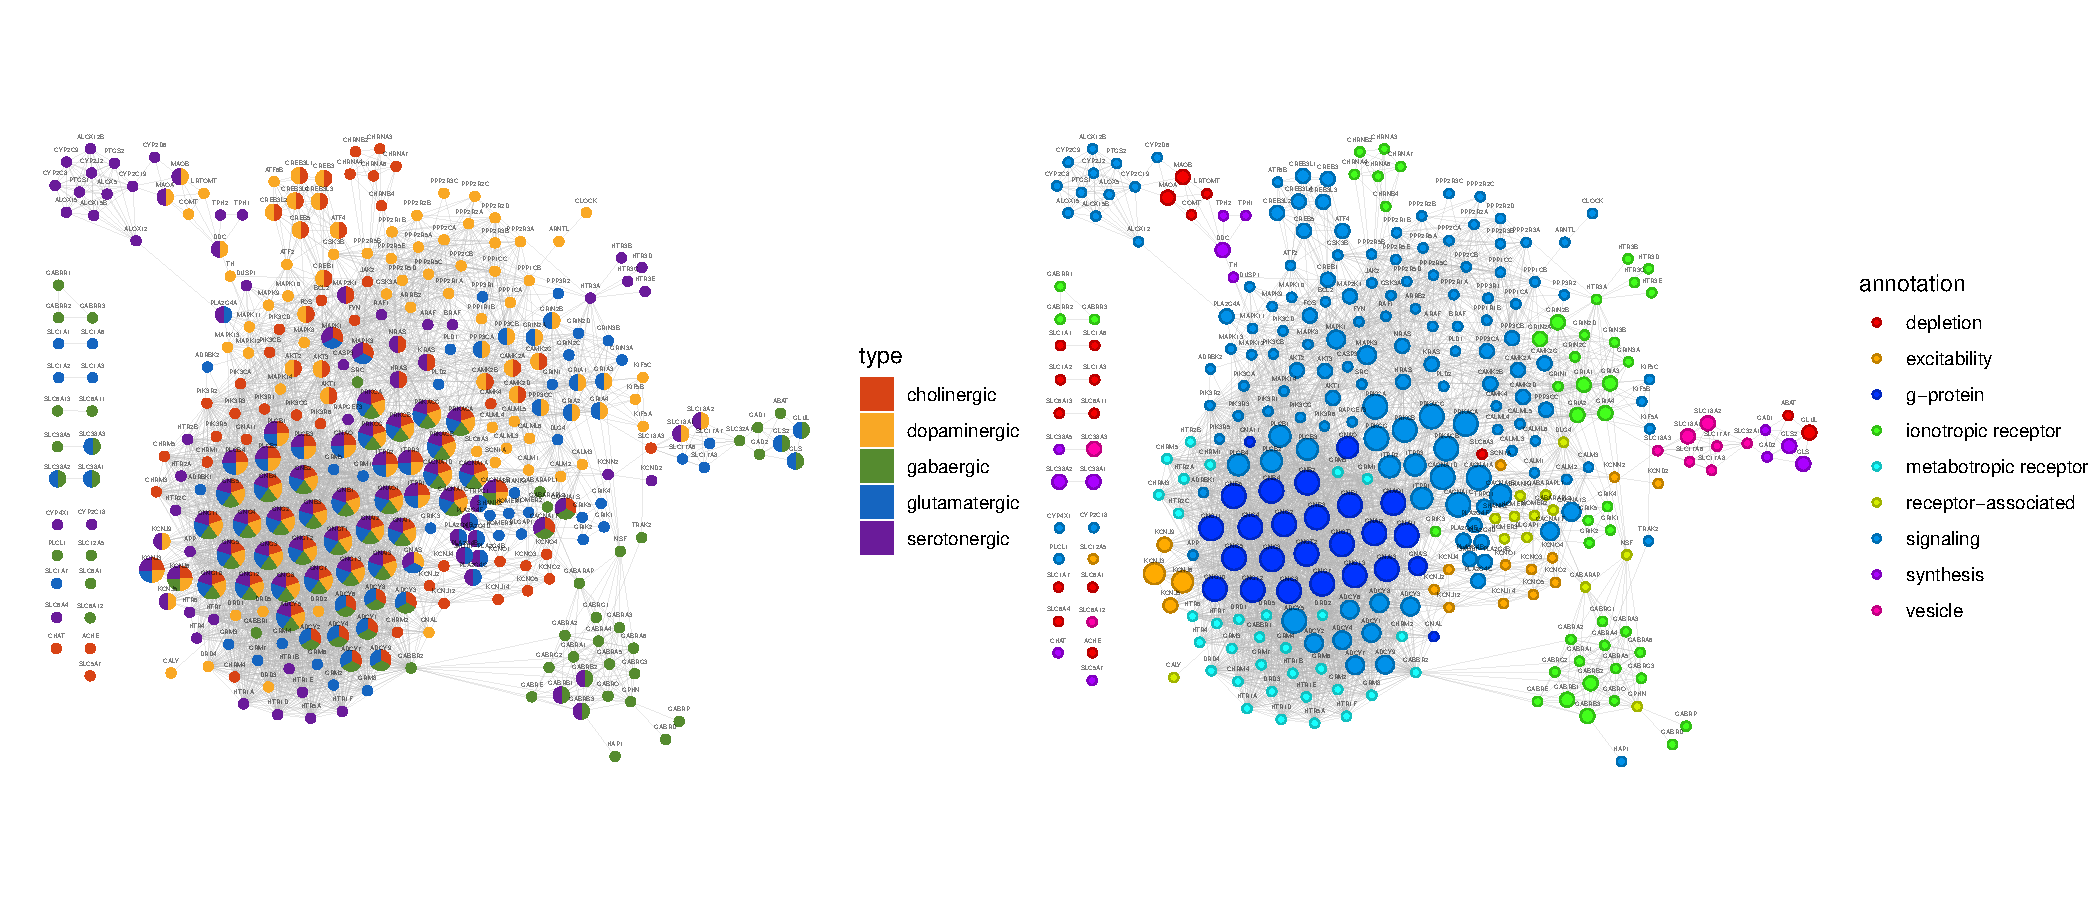
\includegraphics{figs/analysis.network.unnamed-chunk-8-1} 

}

\caption{Unedited manuscript figure 1. The human neurotransmission network with nodes colored by neurotransmitter systems (left) and neurotransmission functions (right).}\label{fig:unnamed-chunk-8}
\end{figure}

\begin{Shaded}
\begin{Highlighting}[]
\KeywordTok{ggsave}\NormalTok{(}\StringTok{"plots/fig1_raw.pdf"}\NormalTok{, }\DataTypeTok{width =} \DecValTok{14}\NormalTok{, }\DataTypeTok{height =} \DecValTok{7}\NormalTok{, }\DataTypeTok{onefile =}\NormalTok{ F, }\DataTypeTok{useDingbats =}\NormalTok{ F)}
\end{Highlighting}
\end{Shaded}

\hypertarget{manuscript-figure-2}{%
\subsubsection{Manuscript figure 2}\label{manuscript-figure-2}}

This figure is produced externally by a program called ViaComplex.
ViaComplex superimposes a heatmap over the network layout based on a
node property. This property, in our case, is a node's neuroexclusivity.
The following block handles data formatting related to ViaComplex.

\begin{Shaded}
\begin{Highlighting}[]
\CommentTok{# Retrieving the largest connected component}
\NormalTok{subgraphs <-}\StringTok{ }\KeywordTok{decompose.graph}\NormalTok{(g)}
\NormalTok{lcc_index <-}\StringTok{ }\KeywordTok{which.max}\NormalTok{(}\KeywordTok{sapply}\NormalTok{(subgraphs, vcount))}
\NormalTok{lcc       <-}\StringTok{ }\NormalTok{subgraphs[[lcc_index]]}

\CommentTok{# Writing network data to viacomplex's custom format (similar to pajek)}
\CommentTok{# xy_hack adds some extra margin to the plot}
\NormalTok{xy_hack <-}\StringTok{ }\KeywordTok{data.frame}\NormalTok{(}
   \DataTypeTok{name                        =} \KeywordTok{c}\NormalTok{(}\StringTok{"top"}\NormalTok{, }\StringTok{"bot"}\NormalTok{)}
\NormalTok{  ,}\DataTypeTok{x                           =} \KeywordTok{range}\NormalTok{(}\KeywordTok{V}\NormalTok{(lcc)}\OperatorTok{$}\NormalTok{x) }\OperatorTok{+}\StringTok{ }\KeywordTok{c}\NormalTok{(}\OperatorTok{-}\DecValTok{75}\NormalTok{, }\DecValTok{75}\NormalTok{)}
\NormalTok{  ,}\DataTypeTok{y                           =} \KeywordTok{range}\NormalTok{(}\KeywordTok{V}\NormalTok{(lcc)}\OperatorTok{$}\NormalTok{y) }\OperatorTok{+}\StringTok{ }\KeywordTok{c}\NormalTok{(}\OperatorTok{-}\DecValTok{75}\NormalTok{, }\DecValTok{75}\NormalTok{)}
\NormalTok{  ,}\DataTypeTok{pathway_neuroexclusivity    =} \DecValTok{0}
\NormalTok{  ,}\DataTypeTok{expression_neuroexclusivity =} \DecValTok{0}
\NormalTok{  ,}\DataTypeTok{stringsAsFactors            =}\NormalTok{ F}
\NormalTok{)}

\NormalTok{pajek_nodes <-}\StringTok{ }\NormalTok{lcc }\OperatorTok
\StringTok{  }\NormalTok{igraph}\OperatorTok{::}\KeywordTok{as_data_frame}\NormalTok{(}\StringTok{"vertices"}\NormalTok{) }\OperatorTok
\StringTok{  }\KeywordTok{bind_rows}\NormalTok{(xy_hack) }\OperatorTok
\StringTok{  }\KeywordTok{mutate}\NormalTok{(}\DataTypeTok{id =} \KeywordTok{row_number}\NormalTok{(), }\DataTypeTok{y =} \OperatorTok{-}\NormalTok{y)}

\NormalTok{pajek_edges <-}\StringTok{ }\NormalTok{igraph}\OperatorTok{::}\KeywordTok{as_data_frame}\NormalTok{(lcc, }\StringTok{"edges"}\NormalTok{)}

\CommentTok{# Creating the network_viacomplex.net file and sequentially populating it}
\KeywordTok{write}\NormalTok{(}\StringTok{"*edges"}\NormalTok{, }\StringTok{"network_viacomplex.net"}\NormalTok{)}
\KeywordTok{write_tsv}\NormalTok{(}
   \DataTypeTok{x            =}\NormalTok{ pajek_edges}
\NormalTok{  ,}\DataTypeTok{path         =} \StringTok{"network_viacomplex.net"}
\NormalTok{  ,}\DataTypeTok{append       =}\NormalTok{ T}
\NormalTok{  ,}\DataTypeTok{col_names    =}\NormalTok{ F}
\NormalTok{  ,}\DataTypeTok{quote_escape =}\NormalTok{ F}
\NormalTok{)}
\KeywordTok{write}\NormalTok{(}\StringTok{"*nodes"}\NormalTok{, }\StringTok{"network_viacomplex.net"}\NormalTok{, }\DataTypeTok{append =}\NormalTok{ T)}
\KeywordTok{write_tsv}\NormalTok{(}
   \DataTypeTok{x            =}\NormalTok{ pajek_nodes }\OperatorTok\StringTok{ }\KeywordTok{select}\NormalTok{(name, x, y)}
\NormalTok{  ,}\DataTypeTok{path         =} \StringTok{"network_viacomplex.net"}
\NormalTok{  ,}\DataTypeTok{append       =}\NormalTok{ T}
\NormalTok{  ,}\DataTypeTok{col_names    =}\NormalTok{ F}
\NormalTok{  ,}\DataTypeTok{quote_escape =}\NormalTok{ F}
\NormalTok{)}

\KeywordTok{write_tsv}\NormalTok{(}
   \DataTypeTok{x    =}\NormalTok{ pajek_nodes }\OperatorTok\StringTok{ }\KeywordTok{select}\NormalTok{(id, name, pathway_neuroexclusivity)}
\NormalTok{  ,}\DataTypeTok{path =} \StringTok{"network_viacomplex_pathway.dat"}
\NormalTok{)}
\KeywordTok{write_tsv}\NormalTok{(}
   \DataTypeTok{x    =}\NormalTok{ pajek_nodes }\OperatorTok\StringTok{ }\KeywordTok{select}\NormalTok{(id, name, expression_neuroexclusivity)}
\NormalTok{  ,}\DataTypeTok{path =} \StringTok{"network_viacomplex_expression.dat"}
\NormalTok{)}
\end{Highlighting}
\end{Shaded}

\hypertarget{manuscript-figure-3}{%
\subsubsection{Manuscript figure 3}\label{manuscript-figure-3}}

The process for generating Figures 3 and 4 is roughly the same. It
consists of finding what nodes have numeric roots in a given range. In
our analysis, the largest root is numbered 37 and represents the oldest
common ancestor to humans in the cladogram (the Human-Metamonada LCA, as
seen in previous sections). Root number 1 is represented by \emph{Homo
sapiens} itself.\\
The nodes we need to draw are either \texttt{current\_nodes} (roots in a
specified numeric range), or \texttt{past\_nodes} (roots \textgreater{}
such specified range). The edges we need to draw are all edges between
both sets of nodes.\\
\textbf{Manuscript Figure 3A}

\begin{Shaded}
\begin{Highlighting}[]
\CommentTok{# Finding which genes should be drawn}
\NormalTok{current_genes <-}\StringTok{ }\NormalTok{vertices }\OperatorTok\StringTok{ }\KeywordTok{filter}\NormalTok{(root }\OperatorTok{==}\StringTok{ }\DecValTok{37}\NormalTok{)}

\CommentTok{# Finding which edges should be drawn}
\NormalTok{partial_ids   <-}\StringTok{ }\NormalTok{current_genes }\OperatorTok\StringTok{ }\KeywordTok{pull}\NormalTok{(string_id)}
\NormalTok{which_edges   <-}\StringTok{ }\KeywordTok{apply}\NormalTok{(string_edgelist, }\DecValTok{1}\NormalTok{, }\ControlFlowTok{function}\NormalTok{(r) }\KeywordTok{all}\NormalTok{(r }\OperatorTok\StringTok{ }\NormalTok{partial_ids))}
\NormalTok{partial_edges <-}\StringTok{ }\NormalTok{edges[which_edges,]}

\NormalTok{plot_edges <-}\StringTok{ }\KeywordTok{geom_path}\NormalTok{(}
   \DataTypeTok{data    =}\NormalTok{ partial_edges}
\NormalTok{  ,}\DataTypeTok{mapping =}\NormalTok{ edge_aes}
\NormalTok{  ,}\DataTypeTok{color   =}\NormalTok{ edge_color}
\NormalTok{  ,}\DataTypeTok{size    =} \FloatTok{0.1}
\NormalTok{)}

\NormalTok{plot_text <-}\StringTok{ }\KeywordTok{geom_text}\NormalTok{(}
   \DataTypeTok{data    =}\NormalTok{ current_genes}
\NormalTok{  ,}\DataTypeTok{mapping =}\NormalTok{ text_aes}
\NormalTok{  ,}\DataTypeTok{size    =} \DecValTok{1}
\NormalTok{  ,}\DataTypeTok{vjust   =} \DecValTok{0}
\NormalTok{  ,}\DataTypeTok{nudge_y =} \FloatTok{1.75}
\NormalTok{  ,}\DataTypeTok{alpha   =} \FloatTok{0.5}
\NormalTok{)}

\NormalTok{plot_current_pies <-}\StringTok{ }\KeywordTok{geom_scatterpie}\NormalTok{(}
   \DataTypeTok{data    =}\NormalTok{ current_genes}
\NormalTok{  ,}\DataTypeTok{mapping =}\NormalTok{ pie_aes}
\NormalTok{  ,}\DataTypeTok{cols    =}\NormalTok{ systems}
\NormalTok{  ,}\DataTypeTok{color   =} \OtherTok{NA}
\NormalTok{)}

\CommentTok{# Assembling}
\NormalTok{fig3a <-}\StringTok{ }\KeywordTok{ggplot}\NormalTok{() }\OperatorTok{+}
\StringTok{  }\NormalTok{plot_edges }\OperatorTok{+}
\StringTok{  }\NormalTok{plot_scales }\OperatorTok{+}
\StringTok{  }\NormalTok{xy_lim }\OperatorTok{+}
\StringTok{  }\NormalTok{plot_current_pies }\OperatorTok{+}
\StringTok{  }\NormalTok{plot_pie_fill }\OperatorTok{+}
\StringTok{  }\NormalTok{plot_text }\OperatorTok{+}
\StringTok{  }\NormalTok{plot_theme}
\end{Highlighting}
\end{Shaded}

\textbf{Manuscript Figure 3B}\\
For Figure 3B, we want to see what nodes have numeric roots \textless{}
37 (Human-Metamonada LCA) and \textgreater= 26 (Human-Cnidaria LCA).

\begin{Shaded}
\begin{Highlighting}[]
\CommentTok{# Finding which genes should be drawn}
\NormalTok{current_genes <-}\StringTok{ }\NormalTok{vertices }\OperatorTok\StringTok{ }\KeywordTok{filter}\NormalTok{(root }\OperatorTok{<}\StringTok{ }\DecValTok{37} \OperatorTok{&}\StringTok{ }\NormalTok{root }\OperatorTok{>=}\StringTok{ }\DecValTok{26}\NormalTok{)}
\NormalTok{past_genes    <-}\StringTok{ }\NormalTok{vertices }\OperatorTok\StringTok{ }\KeywordTok{filter}\NormalTok{(root }\OperatorTok{==}\StringTok{ }\DecValTok{37}\NormalTok{)}

\CommentTok{# Finding which edges should be drawn}
\NormalTok{partial_ids   <-}\StringTok{ }\KeywordTok{c}\NormalTok{(current_genes[[}\StringTok{"string_id"}\NormalTok{]], past_genes[[}\StringTok{"string_id"}\NormalTok{]])}
\NormalTok{which_edges   <-}\StringTok{ }\KeywordTok{apply}\NormalTok{(string_edgelist, }\DecValTok{1}\NormalTok{, }\ControlFlowTok{function}\NormalTok{(r) }\KeywordTok{all}\NormalTok{(r }\OperatorTok\StringTok{ }\NormalTok{partial_ids))}
\NormalTok{partial_edges <-}\StringTok{ }\NormalTok{edges[which_edges,]}

\NormalTok{plot_edges <-}\StringTok{ }\KeywordTok{geom_path}\NormalTok{(}
   \DataTypeTok{data    =}\NormalTok{ partial_edges}
\NormalTok{  ,}\DataTypeTok{mapping =}\NormalTok{ edge_aes}
\NormalTok{  ,}\DataTypeTok{color   =}\NormalTok{ edge_color}
\NormalTok{  ,}\DataTypeTok{size    =} \FloatTok{0.1}
\NormalTok{)}

\NormalTok{plot_past <-}\StringTok{ }\KeywordTok{geom_point}\NormalTok{(}
   \DataTypeTok{data    =}\NormalTok{ past_genes}
\NormalTok{  ,}\DataTypeTok{mapping =} \KeywordTok{aes}\NormalTok{(x, y, }\DataTypeTok{size =}\NormalTok{ size)}
\NormalTok{  ,}\DataTypeTok{fill    =}\NormalTok{ past_fill}
\NormalTok{  ,}\DataTypeTok{color   =}\NormalTok{ past_color}
\NormalTok{  ,}\DataTypeTok{shape   =}\NormalTok{ past_genes}\OperatorTok{$}\NormalTok{shape}
\NormalTok{  ,}\DataTypeTok{stroke  =} \FloatTok{0.25}
\NormalTok{)}

\NormalTok{plot_text <-}\StringTok{ }\KeywordTok{geom_text}\NormalTok{(}
   \DataTypeTok{data    =}\NormalTok{ current_genes}
\NormalTok{  ,}\DataTypeTok{mapping =}\NormalTok{ text_aes}
\NormalTok{  ,}\DataTypeTok{size    =} \DecValTok{1}
\NormalTok{  ,}\DataTypeTok{vjust   =} \DecValTok{0}
\NormalTok{  ,}\DataTypeTok{nudge_y =} \FloatTok{1.75}
\NormalTok{  ,}\DataTypeTok{alpha   =} \FloatTok{0.5}
\NormalTok{)}

\NormalTok{plot_current_pies <-}\StringTok{ }\KeywordTok{geom_scatterpie}\NormalTok{(}
   \DataTypeTok{data    =}\NormalTok{ current_genes}
\NormalTok{  ,}\DataTypeTok{mapping =}\NormalTok{ pie_aes}
\NormalTok{  ,}\DataTypeTok{cols    =}\NormalTok{ systems}
\NormalTok{  ,}\DataTypeTok{color   =} \OtherTok{NA}
\NormalTok{)}

\CommentTok{# Assembling}
\NormalTok{fig3b <-}\StringTok{ }\KeywordTok{ggplot}\NormalTok{() }\OperatorTok{+}
\StringTok{  }\NormalTok{plot_edges }\OperatorTok{+}
\StringTok{  }\NormalTok{plot_past }\OperatorTok{+}
\StringTok{  }\NormalTok{plot_scales }\OperatorTok{+}
\StringTok{  }\NormalTok{xy_lim }\OperatorTok{+}
\StringTok{  }\NormalTok{plot_current_pies }\OperatorTok{+}
\StringTok{  }\NormalTok{plot_pie_fill }\OperatorTok{+}
\StringTok{  }\NormalTok{plot_text }\OperatorTok{+}
\StringTok{  }\NormalTok{plot_theme}

\CommentTok{# Plotting and saving}
\NormalTok{fig3a }\OperatorTok{+}\StringTok{ }\NormalTok{fig3b}
\end{Highlighting}
\end{Shaded}

\begin{figure}

{\centering 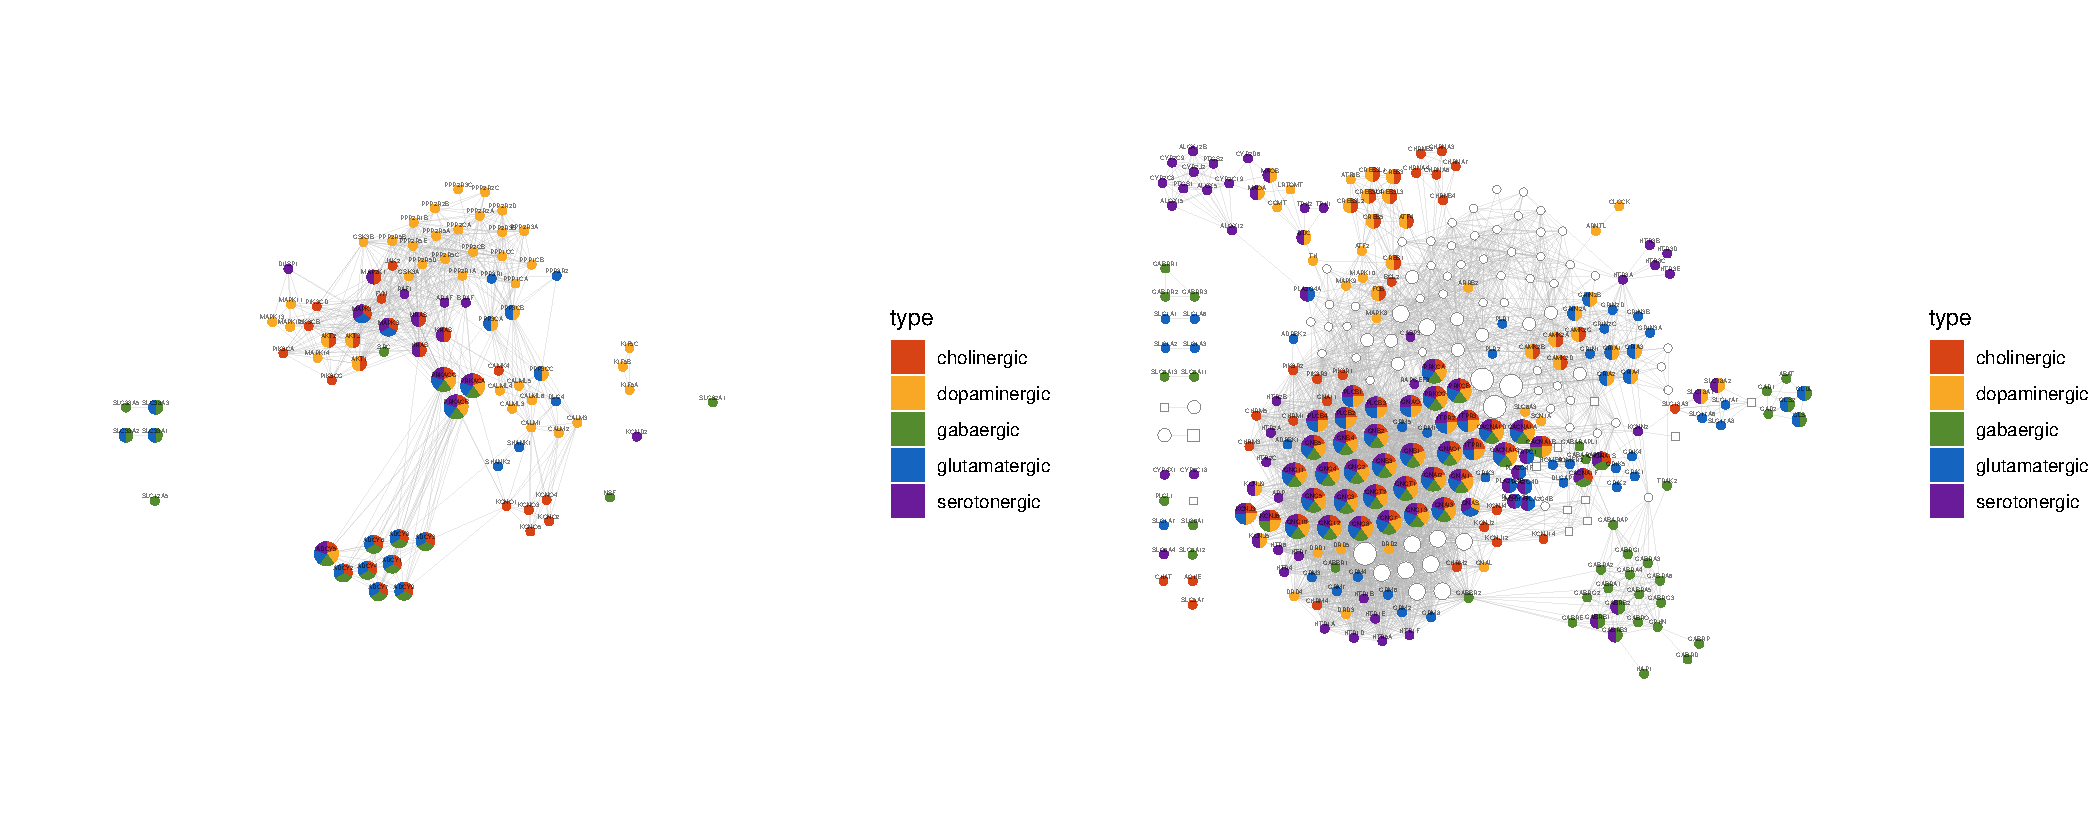
\includegraphics{figs/analysis.network.unnamed-chunk-11-1} 

}

\caption{Unedited manuscript figure 3. The human neurotransmission network with nodes colored by neurotransmitter systems and neurotransmission functions.}\label{fig:unnamed-chunk-11}
\end{figure}

\begin{Shaded}
\begin{Highlighting}[]
\KeywordTok{ggsave}\NormalTok{(}\StringTok{"plots/fig3_raw.pdf"}\NormalTok{, }\DataTypeTok{width =} \DecValTok{14}\NormalTok{, }\DataTypeTok{height =} \DecValTok{7}\NormalTok{, }\DataTypeTok{onefile =}\NormalTok{ F, }\DataTypeTok{useDingbats =}\NormalTok{ F)}
\end{Highlighting}
\end{Shaded}

Additionally, we cumulatively count nodes by their categories (function
and neuroexclusivity) and inferred root:

\begin{Shaded}
\begin{Highlighting}[]
\NormalTok{cumulative_emergence <-}\StringTok{ }\NormalTok{vertices }\OperatorTok
\StringTok{  }\KeywordTok{select}\NormalTok{(root, annotation, }\DataTypeTok{is_neuroexclusive =}\NormalTok{ ne) }\OperatorTok
\StringTok{  }\CommentTok{# Adding clade info}
\StringTok{  }\KeywordTok{right_join}\NormalTok{(clade_names) }\OperatorTok
\StringTok{  }\CommentTok{# Pivoting from wide to long}
\StringTok{  }\KeywordTok{pivot_longer}\NormalTok{(annotation}\OperatorTok{:}\NormalTok{is_neuroexclusive, }\DataTypeTok{values_ptypes =} \KeywordTok{list}\NormalTok{(}\DataTypeTok{value =} \StringTok{"character"}\NormalTok{)) }\OperatorTok
\StringTok{  }\CommentTok{# Counting nodes by category (name) for each root}
\StringTok{  }\KeywordTok{count}\NormalTok{(root, clade_name, name, value) }\OperatorTok
\StringTok{  }\CommentTok{# Making absent counts explicit}
\StringTok{  }\KeywordTok{group_by}\NormalTok{(name) }\OperatorTok
\StringTok{  }\KeywordTok{complete}\NormalTok{(}\KeywordTok{nesting}\NormalTok{(root, clade_name), name, value, }\DataTypeTok{fill =} \KeywordTok{list}\NormalTok{(}\DataTypeTok{n =} \DecValTok{0}\NormalTok{)) }\OperatorTok
\StringTok{  }\CommentTok{# No reason to include NA observations in cumulative sum}
\StringTok{  }\NormalTok{na.omit }\OperatorTok
\StringTok{  }\CommentTok{# Cumulative sum node count at each root}
\StringTok{  }\KeywordTok{group_by}\NormalTok{(name, value) }\OperatorTok
\StringTok{  }\KeywordTok{mutate}\NormalTok{(}\DataTypeTok{cumulative_count =} \KeywordTok{order_by}\NormalTok{(}\OperatorTok{-}\NormalTok{root, }\KeywordTok{cumsum}\NormalTok{(n)))}
\end{Highlighting}
\end{Shaded}

Plotting such cumulative counts:

\begin{Shaded}
\begin{Highlighting}[]
\NormalTok{cumulative_emergence }\OperatorTok\StringTok{ }\NormalTok{ungroup }\OperatorTok
\StringTok{  }\CommentTok{# Creating ordered factors for plotting}
\StringTok{  }\KeywordTok{mutate}\NormalTok{(}
     \DataTypeTok{clade_name =} \KeywordTok{fct_reorder}\NormalTok{(clade_name, }\OperatorTok{-}\NormalTok{root)}
\NormalTok{    ,}\DataTypeTok{value      =} \KeywordTok{fct_reorder}\NormalTok{(value, name)}
\NormalTok{  )}

\KeywordTok{ggplot}\NormalTok{(cumulative_emergence) }\OperatorTok{+}
\StringTok{  }\CommentTok{#----- Barplot ------}
\StringTok{  }\KeywordTok{geom_bar}\NormalTok{(}
     \DataTypeTok{mapping     =} \KeywordTok{aes}\NormalTok{(clade_name, cumulative_count, }\DataTypeTok{group =}\NormalTok{ value)}
\NormalTok{    ,}\DataTypeTok{stat        =} \StringTok{"sum"}
\NormalTok{    ,}\DataTypeTok{fill        =} \StringTok{"#999999"}
\NormalTok{    ,}\DataTypeTok{show.legend =}\NormalTok{ F}
\NormalTok{  ) }\OperatorTok{+}
\StringTok{  }\CommentTok{#----- Lines ------}
\StringTok{  }\KeywordTok{geom_line}\NormalTok{(}
     \DataTypeTok{mapping =} \KeywordTok{aes}\NormalTok{(clade_name, cumulative_count, }\DataTypeTok{group =}\NormalTok{ value, }\DataTypeTok{color =}\NormalTok{ value)}
\NormalTok{    ,}\DataTypeTok{size    =} \DecValTok{1}
\NormalTok{  ) }\OperatorTok{+}
\StringTok{  }\CommentTok{#----- Styling ------}
\StringTok{  }\KeywordTok{scale_color_manual}\NormalTok{(}\DataTypeTok{values =}\NormalTok{ element_colors) }\OperatorTok{+}
\StringTok{  }\KeywordTok{facet_grid}\NormalTok{(name }\OperatorTok{~}\StringTok{ }\NormalTok{.) }\OperatorTok{+}
\StringTok{  }\KeywordTok{theme}\NormalTok{(}\DataTypeTok{axis.text.x =} \KeywordTok{element_text}\NormalTok{(}\DataTypeTok{angle =} \DecValTok{45}\NormalTok{, }\DataTypeTok{vjust =} \DecValTok{1}\NormalTok{, }\DataTypeTok{hjust =} \DecValTok{1}\NormalTok{))}
\end{Highlighting}
\end{Shaded}

\begin{figure}

{\centering 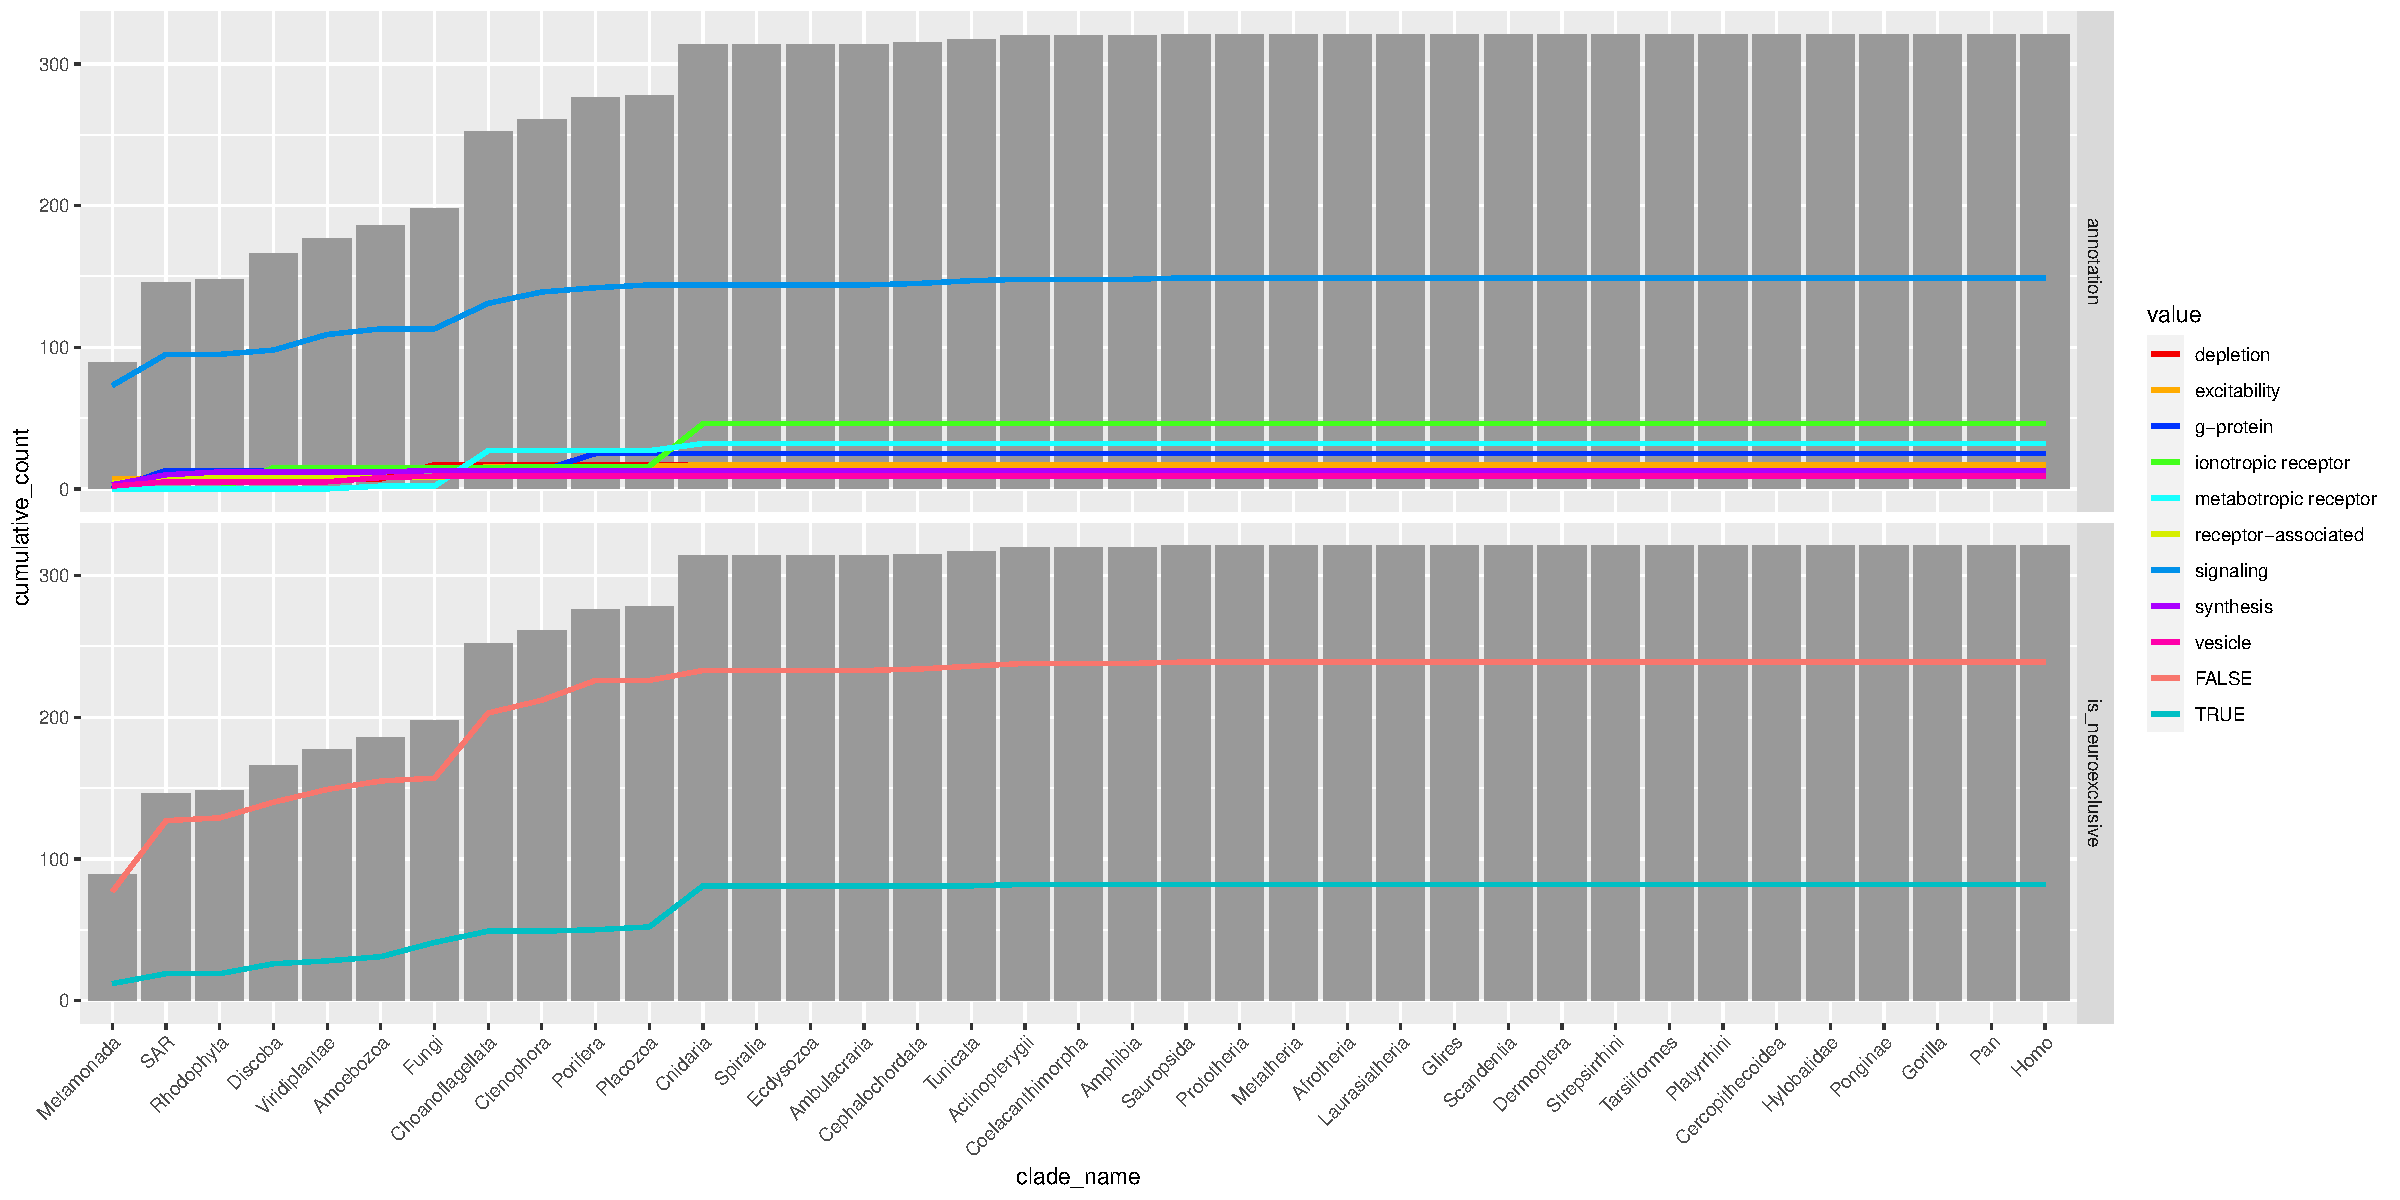
\includegraphics{figs/analysis.network.unnamed-chunk-13-1} 

}

\caption{Cumulative node counts by categories at each root.}\label{fig:unnamed-chunk-13}
\end{figure}

\hypertarget{manuscript-figure-4}{%
\subsubsection{Manuscript figure 4}\label{manuscript-figure-4}}

Visualizing nodes with roots \textless= 30 (Human-Porifera LCA) and
\textgreater= 26 (Human-Cnidaria LCA) at every distinct root.

\begin{Shaded}
\begin{Highlighting}[]
\NormalTok{plot_size <-}\StringTok{ }\KeywordTok{scale_radius}\NormalTok{(}\DataTypeTok{range =} \KeywordTok{c}\NormalTok{(}\FloatTok{0.5}\NormalTok{, }\FloatTok{1.5}\NormalTok{), }\DataTypeTok{guide =} \OtherTok{FALSE}\NormalTok{)}

\NormalTok{fig4 <-}\StringTok{ }\NormalTok{roots[roots }\OperatorTok{>=}\StringTok{ }\DecValTok{26} \OperatorTok{&}\StringTok{ }\NormalTok{roots }\OperatorTok{<=}\StringTok{ }\DecValTok{30}\NormalTok{] }\OperatorTok
\StringTok{  }\KeywordTok{imap}\NormalTok{(}\OperatorTok{~}\StringTok{ }\NormalTok{\{}
  \CommentTok{# Finding which genes should be drawn}
\NormalTok{  current_genes <-}\StringTok{ }\NormalTok{vertices }\OperatorTok\StringTok{ }\KeywordTok{filter}\NormalTok{(root }\OperatorTok{==}\StringTok{ }\NormalTok{.x)}
\NormalTok{  past_genes    <-}\StringTok{ }\NormalTok{vertices }\OperatorTok\StringTok{ }\KeywordTok{filter}\NormalTok{(root  }\OperatorTok{>}\StringTok{ }\NormalTok{.x)}
  
  \CommentTok{# Finding which edges should be drawn}
\NormalTok{  partial_ids   <-}\StringTok{ }\KeywordTok{c}\NormalTok{(current_genes[[}\StringTok{"string_id"}\NormalTok{]], past_genes[[}\StringTok{"string_id"}\NormalTok{]])}
\NormalTok{  which_edges   <-}\StringTok{ }\KeywordTok{apply}\NormalTok{(string_edgelist, }\DecValTok{1}\NormalTok{, }\ControlFlowTok{function}\NormalTok{(r) }\KeywordTok{all}\NormalTok{(r }\OperatorTok\StringTok{ }\NormalTok{partial_ids))}
\NormalTok{  partial_edges <-}\StringTok{ }\NormalTok{edges[which_edges,]}
  
\NormalTok{  plot_edges <-}\StringTok{ }\KeywordTok{geom_path}\NormalTok{(}
     \DataTypeTok{data    =}\NormalTok{ partial_edges}
\NormalTok{    ,}\DataTypeTok{mapping =}\NormalTok{ edge_aes}
\NormalTok{    ,}\DataTypeTok{color   =}\NormalTok{ edge_color}
\NormalTok{    ,}\DataTypeTok{size    =} \FloatTok{0.1}
\NormalTok{  )}
  
\NormalTok{  plot_past <-}\StringTok{ }\KeywordTok{geom_point}\NormalTok{(}
     \DataTypeTok{data    =}\NormalTok{ past_genes}
\NormalTok{    ,}\DataTypeTok{mapping =} \KeywordTok{aes}\NormalTok{(x, y, }\DataTypeTok{size =}\NormalTok{ size)}
\NormalTok{    ,}\DataTypeTok{fill    =}\NormalTok{ past_fill}
\NormalTok{    ,}\DataTypeTok{color   =}\NormalTok{ past_color}
\NormalTok{    ,}\DataTypeTok{shape   =}\NormalTok{ past_genes}\OperatorTok{$}\NormalTok{shape}
\NormalTok{    ,}\DataTypeTok{stroke  =} \FloatTok{0.25}
\NormalTok{  )}
  
\NormalTok{  plot_text <-}\StringTok{ }\KeywordTok{geom_text}\NormalTok{(}
     \DataTypeTok{data    =}\NormalTok{ current_genes}
\NormalTok{    ,}\DataTypeTok{mapping =}\NormalTok{ text_aes}
\NormalTok{    ,}\DataTypeTok{size    =} \FloatTok{0.8}
\NormalTok{    ,}\DataTypeTok{vjust   =} \FloatTok{-0.5}
\NormalTok{    ,}\DataTypeTok{nudge_y =} \DecValTok{1}
\NormalTok{    ,}\DataTypeTok{alpha   =} \FloatTok{0.5}
\NormalTok{  )}
  
\NormalTok{  plot_current_nodes <-}\StringTok{ }\KeywordTok{geom_point}\NormalTok{(}
     \DataTypeTok{data    =}\NormalTok{ current_genes}
\NormalTok{    ,}\DataTypeTok{mapping =} \KeywordTok{aes}\NormalTok{(x, y, }\DataTypeTok{fill =}\NormalTok{ annotation, }\DataTypeTok{size =}\NormalTok{ size)}
\NormalTok{    ,}\DataTypeTok{color   =}\NormalTok{ current_genes}\OperatorTok{$}\NormalTok{color_node}
\NormalTok{    ,}\DataTypeTok{shape   =}\NormalTok{ current_genes}\OperatorTok{$}\NormalTok{shape}
\NormalTok{    ,}\DataTypeTok{stroke  =} \FloatTok{0.25}
\NormalTok{  )}
  
\NormalTok{  remove_legend <-}\StringTok{ }\KeywordTok{guides}\NormalTok{(}\DataTypeTok{fill =} \StringTok{"none"}\NormalTok{, }\DataTypeTok{colour =} \StringTok{"none"}\NormalTok{)}
  
  \CommentTok{# Assembling}
  \KeywordTok{ggplot}\NormalTok{() }\OperatorTok{+}
\StringTok{    }\KeywordTok{ggtitle}\NormalTok{(}\KeywordTok{paste}\NormalTok{(.y, }\StringTok{"LCA"}\NormalTok{)) }\OperatorTok{+}
\StringTok{    }\NormalTok{diff_theme }\OperatorTok{+}
\StringTok{    }\NormalTok{xy_lim }\OperatorTok{+}
\StringTok{    }\NormalTok{plot_edges }\OperatorTok{+}
\StringTok{    }\NormalTok{plot_past }\OperatorTok{+}
\StringTok{    }\NormalTok{plot_current_nodes }\OperatorTok{+}
\StringTok{    }\NormalTok{plot_scales }\OperatorTok{+}
\StringTok{    }\NormalTok{plot_size }\OperatorTok{+}
\StringTok{    }\NormalTok{plot_text }\OperatorTok{+}
\StringTok{    }\NormalTok{remove_legend}
\NormalTok{\})}

\NormalTok{fig4 <-}\StringTok{ }\KeywordTok{invoke}\NormalTok{(grid.arrange, fig4, }\DataTypeTok{ncol =} \DecValTok{5}\NormalTok{)}
\end{Highlighting}
\end{Shaded}

\begin{figure}

{\centering 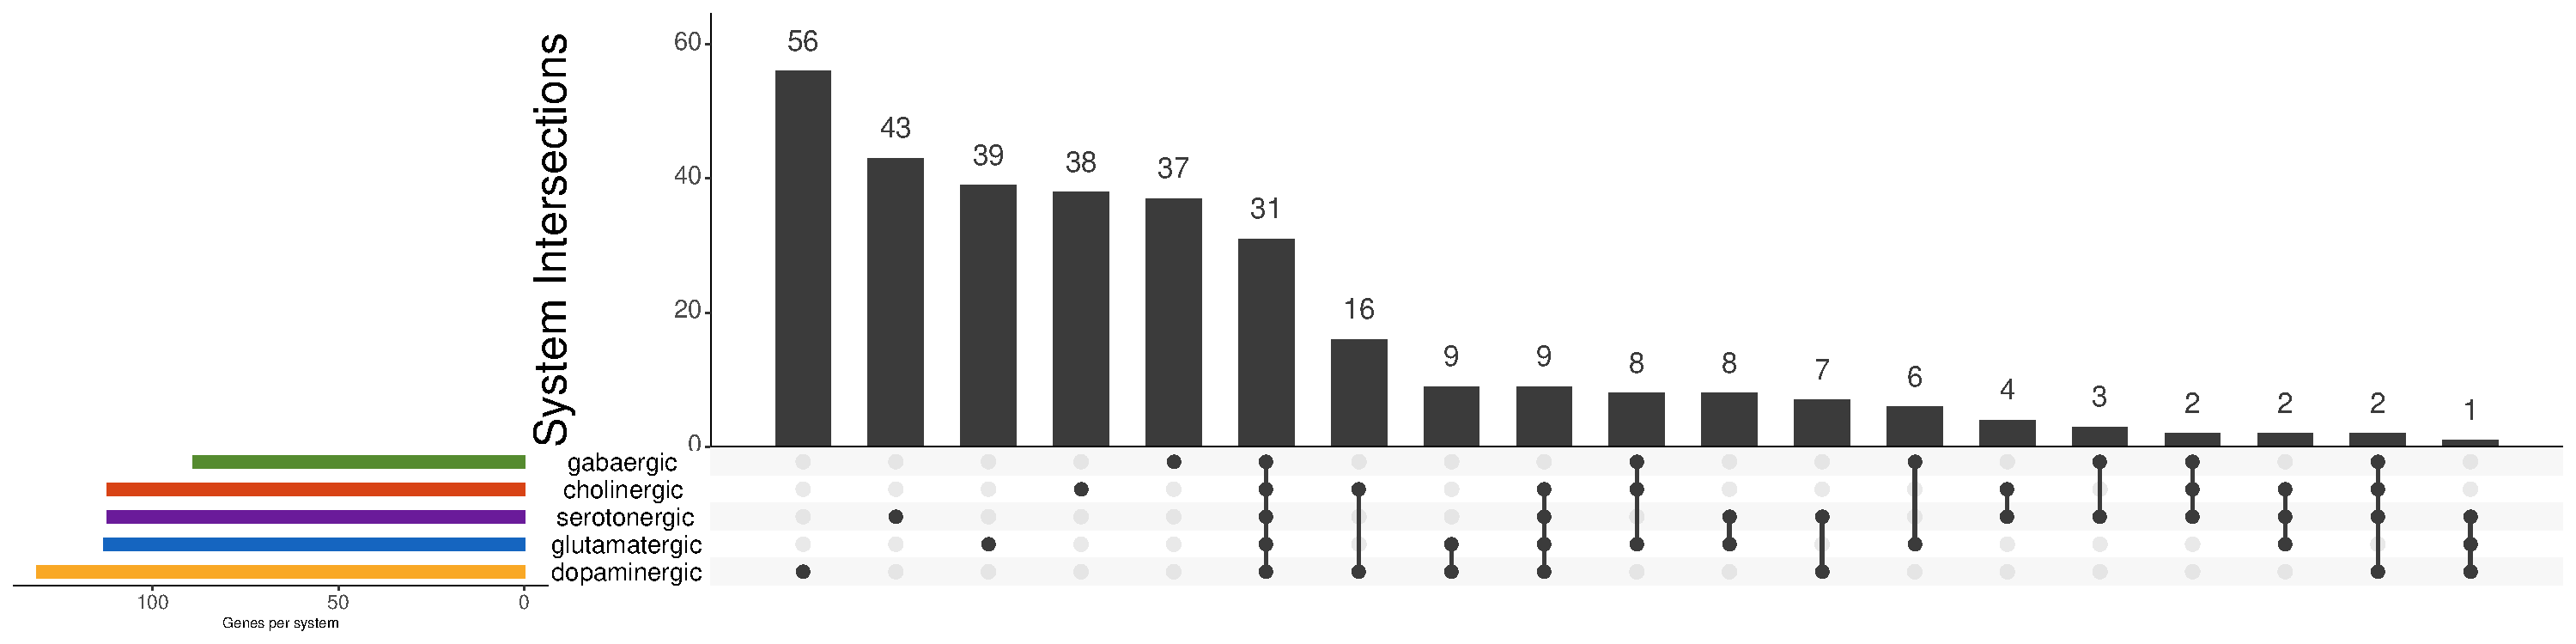
\includegraphics{figs/analysis.network.unnamed-chunk-14-1} 

}

\caption{Unedited manuscript figure 4. The human neurotransmission network with nodes rooted between roots 30 (Human-Choanoflagellata LCA) and 26 (Human-Cnidaria LCA).}\label{fig:unnamed-chunk-14}
\end{figure}

\begin{Shaded}
\begin{Highlighting}[]
\KeywordTok{ggsave}\NormalTok{(}
  \StringTok{"plots/fig4_raw.pdf"}
\NormalTok{  ,}\DataTypeTok{plot        =}\NormalTok{ fig4}
\NormalTok{  ,}\DataTypeTok{width       =} \DecValTok{9}\OperatorTok{*}\FloatTok{0.9}
\NormalTok{  ,}\DataTypeTok{height      =} \DecValTok{5}\OperatorTok{*}\FloatTok{0.9}
\NormalTok{  ,}\DataTypeTok{onefile     =}\NormalTok{ F}
\NormalTok{  ,}\DataTypeTok{useDingbats =}\NormalTok{ F}
\NormalTok{)}
\end{Highlighting}
\end{Shaded}

\hypertarget{supplementary-network-figures}{%
\subsubsection{Supplementary network
figures}\label{supplementary-network-figures}}

The following supplementary figures help us see what nodes have been
rooted at each LCA. Nodes rooted at previous LCAs are colored white.

\begin{Shaded}
\begin{Highlighting}[]
\NormalTok{system_plots   <-}\StringTok{ }\KeywordTok{list}\NormalTok{()}
\NormalTok{function_plots <-}\StringTok{ }\KeywordTok{list}\NormalTok{()}

\KeywordTok{iwalk}\NormalTok{(roots, }\OperatorTok{~}\StringTok{ }\NormalTok{\{}
  \CommentTok{# Finding which genes should be drawn}
\NormalTok{  current_genes <-}\StringTok{ }\NormalTok{vertices }\OperatorTok\StringTok{ }\KeywordTok{filter}\NormalTok{(root }\OperatorTok{==}\StringTok{ }\NormalTok{.x)}
\NormalTok{  past_genes    <-}\StringTok{ }\NormalTok{vertices }\OperatorTok\StringTok{ }\KeywordTok{filter}\NormalTok{(root  }\OperatorTok{>}\StringTok{ }\NormalTok{.x)}
  
  \CommentTok{# Finding which edges should be drawn}
\NormalTok{  partial_ids   <-}\StringTok{ }\KeywordTok{c}\NormalTok{(current_genes[[}\StringTok{"string_id"}\NormalTok{]], past_genes[[}\StringTok{"string_id"}\NormalTok{]])}
\NormalTok{  which_edges   <-}\StringTok{ }\KeywordTok{apply}\NormalTok{(string_edgelist, }\DecValTok{1}\NormalTok{, }\ControlFlowTok{function}\NormalTok{(r) }\KeywordTok{all}\NormalTok{(r }\OperatorTok\StringTok{ }\NormalTok{partial_ids))}
\NormalTok{  partial_edges <-}\StringTok{ }\NormalTok{edges[which_edges,]}
  
  \CommentTok{# Common elements -----------}
\NormalTok{  plot_edges <-}\StringTok{ }\KeywordTok{geom_path}\NormalTok{(}
     \DataTypeTok{data    =}\NormalTok{ partial_edges}
\NormalTok{    ,}\DataTypeTok{mapping =}\NormalTok{ edge_aes}
\NormalTok{    ,}\DataTypeTok{color   =}\NormalTok{ edge_color}
\NormalTok{    ,}\DataTypeTok{size    =} \FloatTok{0.1}
\NormalTok{  )}
  
\NormalTok{  plot_past <-}\StringTok{ }\KeywordTok{geom_point}\NormalTok{(}
     \DataTypeTok{data    =}\NormalTok{ past_genes}
\NormalTok{    ,}\DataTypeTok{mapping =} \KeywordTok{aes}\NormalTok{(x, y, }\DataTypeTok{size =}\NormalTok{ size)}
\NormalTok{    ,}\DataTypeTok{fill    =}\NormalTok{ past_fill}
\NormalTok{    ,}\DataTypeTok{color   =}\NormalTok{ past_color}
\NormalTok{    ,}\DataTypeTok{shape   =}\NormalTok{ past_genes}\OperatorTok{$}\NormalTok{shape}
\NormalTok{    ,}\DataTypeTok{stroke  =} \FloatTok{0.25}
\NormalTok{  )}
  
\NormalTok{  plot_text <-}\StringTok{ }\KeywordTok{geom_text}\NormalTok{(}\DataTypeTok{data =}\NormalTok{ current_genes, text_aes, }\DataTypeTok{size =} \DecValTok{1}\NormalTok{, }\DataTypeTok{nudge_y =} \DecValTok{2}\NormalTok{, }\DataTypeTok{alpha =} \FloatTok{0.5}\NormalTok{)}
  
\NormalTok{  base <-}\StringTok{ }\KeywordTok{ggplot}\NormalTok{() }\OperatorTok{+}
\StringTok{    }\KeywordTok{ggtitle}\NormalTok{(}\KeywordTok{paste0}\NormalTok{(}\StringTok{"Human-"}\NormalTok{, .y, }\StringTok{" LCA (#"}\NormalTok{, .x, }\StringTok{")"}\NormalTok{)) }\OperatorTok{+}
\StringTok{    }\NormalTok{diff_theme }\OperatorTok{+}
\StringTok{    }\NormalTok{xy_lim }\OperatorTok{+}
\StringTok{    }\NormalTok{plot_edges }\OperatorTok{+}
\StringTok{    }\NormalTok{plot_past }\OperatorTok{+}
\StringTok{    }\NormalTok{plot_size}
  
  \CommentTok{# Nodes colored by system -----------}
\NormalTok{  plot_current_pies <-}\StringTok{ }\KeywordTok{geom_scatterpie}\NormalTok{(}\DataTypeTok{data =}\NormalTok{ current_genes, pie_aes, }\DataTypeTok{cols =}\NormalTok{ systems, }\DataTypeTok{color =} \OtherTok{NA}\NormalTok{)}
  
\NormalTok{  system_plots[[}\KeywordTok{as.character}\NormalTok{(.x)]] <<-}\StringTok{ }\NormalTok{base }\OperatorTok{+}
\StringTok{    }\NormalTok{plot_current_pies }\OperatorTok{+}
\StringTok{    }\NormalTok{plot_pie_fill }\OperatorTok{+}
\StringTok{    }\NormalTok{plot_text}
  
  \CommentTok{# Nodes colored by function --------}
\NormalTok{  plot_current_nodes <-}\StringTok{ }\KeywordTok{geom_point}\NormalTok{(}
     \DataTypeTok{data    =}\NormalTok{ current_genes}
\NormalTok{    ,}\DataTypeTok{mapping =} \KeywordTok{aes}\NormalTok{(x, y, }\DataTypeTok{fill =}\NormalTok{ annotation, }\DataTypeTok{size =}\NormalTok{ size)}
\NormalTok{    ,}\DataTypeTok{color   =}\NormalTok{ current_genes}\OperatorTok{$}\NormalTok{color_node}
\NormalTok{    ,}\DataTypeTok{shape   =}\NormalTok{ current_genes}\OperatorTok{$}\NormalTok{shape}
\NormalTok{    ,}\DataTypeTok{stroke  =} \FloatTok{0.25}
\NormalTok{  )}
  
\NormalTok{  function_plots[[}\KeywordTok{as.character}\NormalTok{(.x)]] <<-}\StringTok{ }\NormalTok{base }\OperatorTok{+}
\StringTok{    }\NormalTok{plot_current_nodes }\OperatorTok{+}
\StringTok{    }\NormalTok{plot_scales }\OperatorTok{+}
\StringTok{    }\NormalTok{plot_size }\OperatorTok{+}
\StringTok{    }\NormalTok{plot_text }\OperatorTok{+}
\StringTok{    }\KeywordTok{guides}\NormalTok{(}\DataTypeTok{fill =} \KeywordTok{guide_legend}\NormalTok{(}\DataTypeTok{override.aes =} \KeywordTok{list}\NormalTok{(}\DataTypeTok{shape =} \DecValTok{21}\NormalTok{))) }\CommentTok{# legend hack}
\NormalTok{\})}

\CommentTok{# Printing and saving}
\KeywordTok{arrangeGrob}\NormalTok{(}\DataTypeTok{grobs =}\NormalTok{ system_plots, }\DataTypeTok{ncol =} \DecValTok{3}\NormalTok{) }\OperatorTok\StringTok{ }\NormalTok{grid}\OperatorTok{::}\KeywordTok{grid.draw}\NormalTok{()}
\end{Highlighting}
\end{Shaded}

\begin{figure}

{\centering 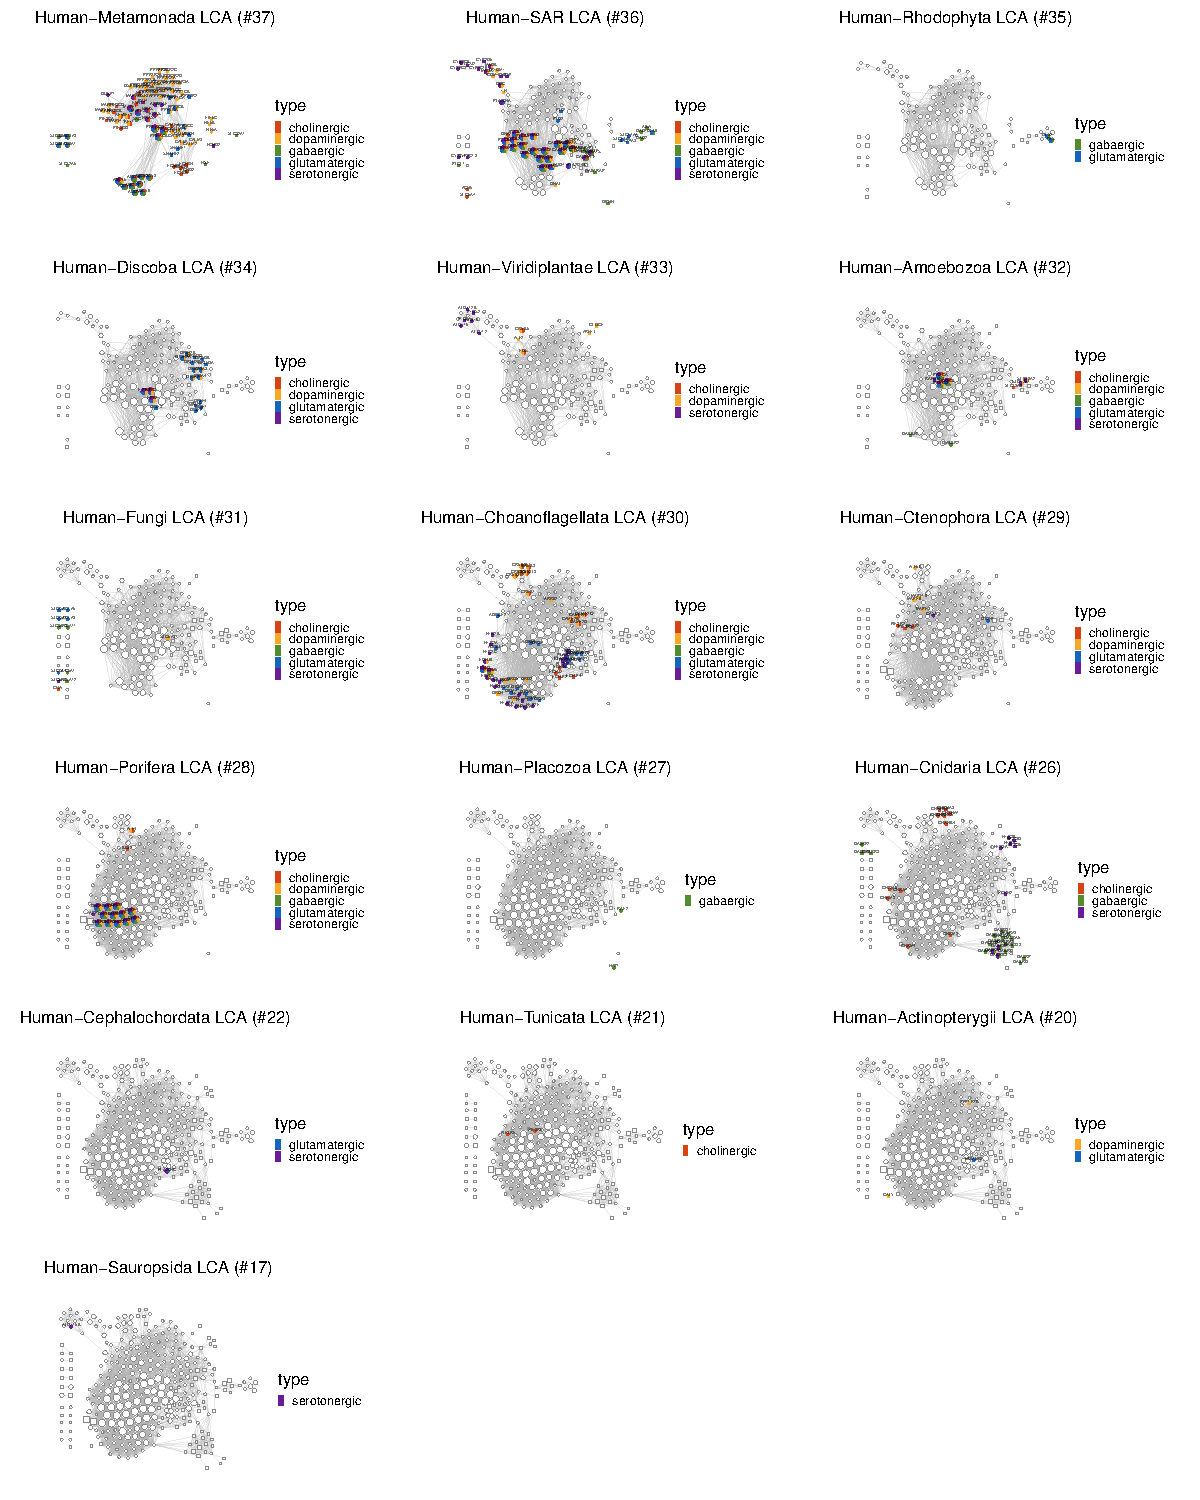
\includegraphics{figs/analysis.network.unnamed-chunk-15-1} 

}

\caption{The human neurotransmission network with nodes rooted at each human LCA.}\label{fig:unnamed-chunk-15}
\end{figure}

\begin{Shaded}
\begin{Highlighting}[]
\KeywordTok{arrangeGrob}\NormalTok{(}\DataTypeTok{grobs =}\NormalTok{ function_plots, }\DataTypeTok{ncol =} \DecValTok{3}\NormalTok{) }\OperatorTok\StringTok{ }\NormalTok{grid}\OperatorTok{::}\KeywordTok{grid.draw}\NormalTok{()}
\end{Highlighting}
\end{Shaded}

\begin{figure}

{\centering 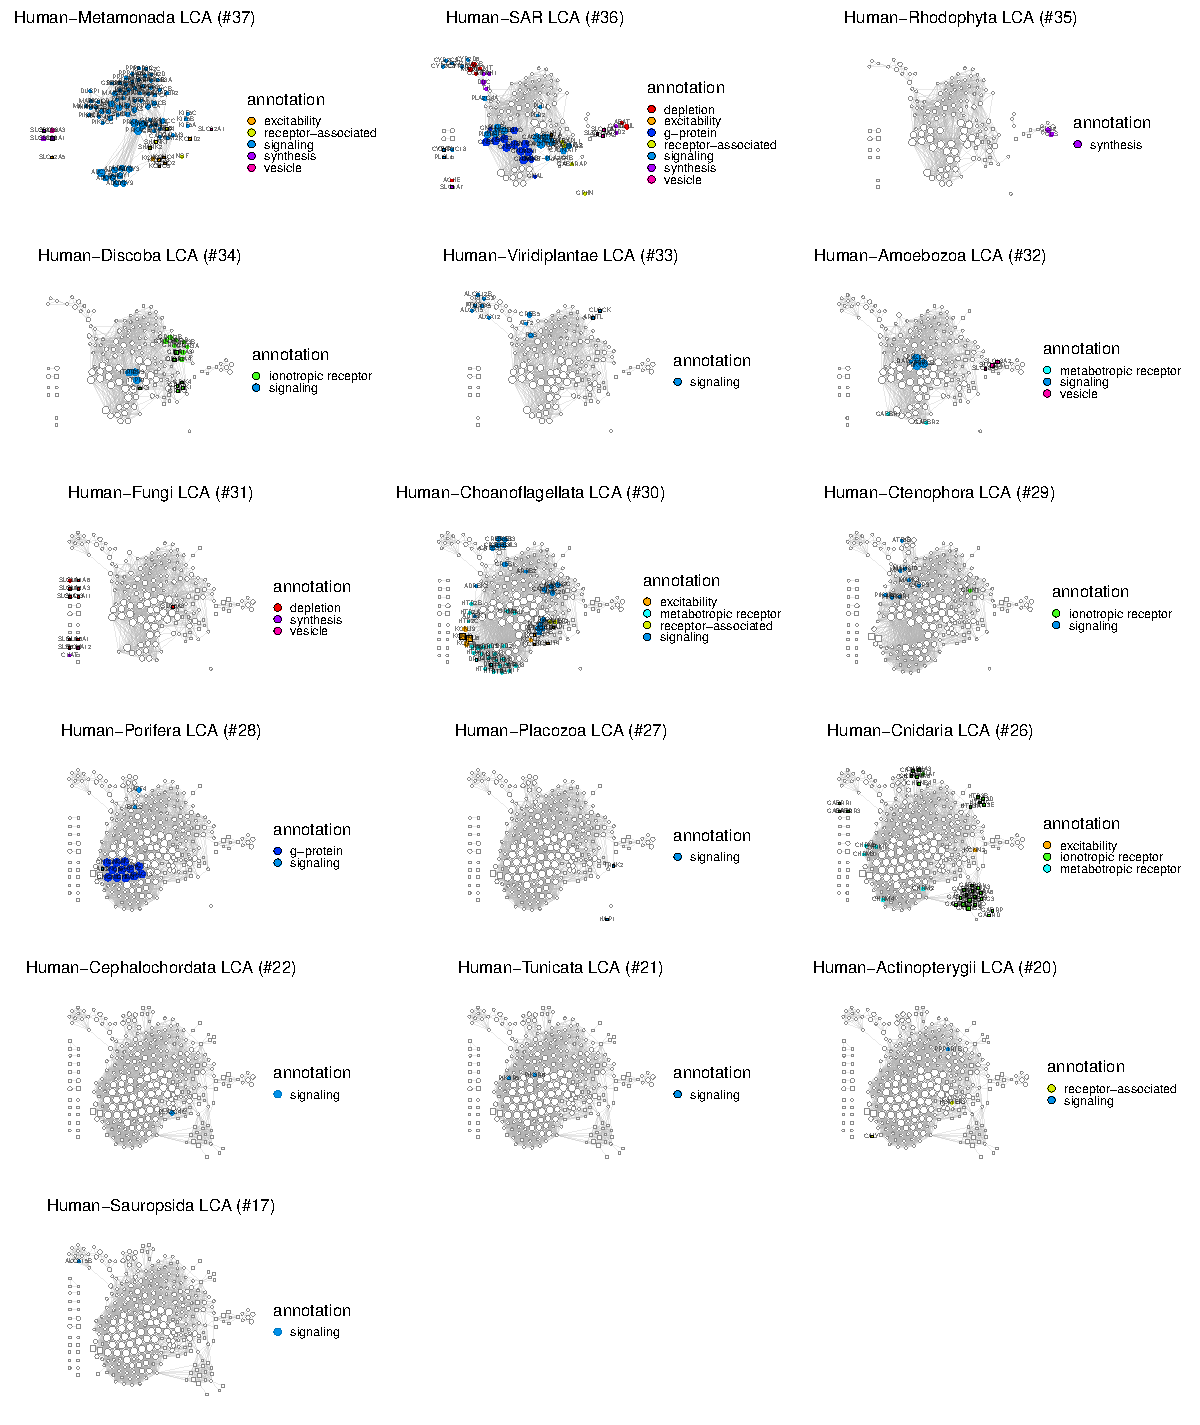
\includegraphics{figs/analysis.network.unnamed-chunk-16-1} 

}

\caption{The human neurotransmission network with nodes rooted at each human LCA.}\label{fig:unnamed-chunk-16}
\end{figure}

\hypertarget{manuscript-set-diagrams}{%
\subsubsection{Manuscript set diagrams}\label{manuscript-set-diagrams}}

Given the dificulties of joining ggplot and base plots, the set diagrams
have to be plotted by themselves:

\begin{Shaded}
\begin{Highlighting}[]
\CommentTok{# We have to manually find the correct order of colors}
\CommentTok{# Because UpSetR does not understand named vectors}
\NormalTok{get_colors <-}\StringTok{ }\ControlFlowTok{function}\NormalTok{(df) \{}
\NormalTok{  ordered_systems <-}\StringTok{ }\NormalTok{df }\OperatorTok
\StringTok{    }\KeywordTok{select}\NormalTok{(systems) }\OperatorTok
\StringTok{    }\NormalTok{colSums }\OperatorTok
\StringTok{    }\KeywordTok{extract}\NormalTok{(. }\OperatorTok{>}\StringTok{ }\DecValTok{0}\NormalTok{) }\OperatorTok
\StringTok{    }\KeywordTok{extract}\NormalTok{(}\KeywordTok{order}\NormalTok{(., }\KeywordTok{names}\NormalTok{(.), }\DataTypeTok{decreasing =}\NormalTok{ T))}

\NormalTok{  pie_colors[}\KeywordTok{names}\NormalTok{(ordered_systems)]}
\NormalTok{\}}

\CommentTok{# Figure 1A set diagram}
\KeywordTok{upset}\NormalTok{(}
   \KeywordTok{select}\NormalTok{(vertices, systems)}
\NormalTok{  ,}\DataTypeTok{mb.ratio        =} \KeywordTok{c}\NormalTok{(}\FloatTok{0.7}\NormalTok{, }\FloatTok{0.3}\NormalTok{)}
\NormalTok{  ,}\DataTypeTok{order.by        =} \StringTok{"freq"}
\NormalTok{  ,}\DataTypeTok{mainbar.y.label =} \StringTok{"System Intersections"}
\NormalTok{  ,}\DataTypeTok{sets.x.label    =} \StringTok{"Genes per system"}
\NormalTok{  ,}\DataTypeTok{text.scale      =}\NormalTok{ upset_texts}
\NormalTok{  ,}\DataTypeTok{point.size      =} \FloatTok{3.5}
\NormalTok{  ,}\DataTypeTok{line.size       =} \DecValTok{1}
\NormalTok{  ,}\DataTypeTok{sets.bar.color  =} \KeywordTok{get_colors}\NormalTok{(vertices)}
\NormalTok{)}
\KeywordTok{dev.print}\NormalTok{(pdf, }\StringTok{"plots/fig1a_set_raw.pdf"}\NormalTok{, }\DataTypeTok{width =} \DecValTok{18}\NormalTok{, }\DataTypeTok{height =} \DecValTok{10}\NormalTok{, }\DataTypeTok{onefile =}\NormalTok{ F, }\DataTypeTok{useDingbats =}\NormalTok{ F)}

\CommentTok{# Figure 3A set diagram}
\NormalTok{fig3a_set <-}\StringTok{ }\NormalTok{vertices }\OperatorTok\StringTok{ }\KeywordTok{filter}\NormalTok{(root }\OperatorTok{==}\StringTok{ }\DecValTok{37}\NormalTok{) }\OperatorTok\StringTok{ }\KeywordTok{select}\NormalTok{(systems)}
\KeywordTok{upset}\NormalTok{(}
\NormalTok{   fig3a_set}
\NormalTok{  ,}\DataTypeTok{mb.ratio        =} \KeywordTok{c}\NormalTok{(}\FloatTok{0.7}\NormalTok{, }\FloatTok{0.3}\NormalTok{)}
\NormalTok{  ,}\DataTypeTok{order.by        =} \StringTok{"freq"}
\NormalTok{  ,}\DataTypeTok{mainbar.y.label =} \StringTok{"System Intersections"}
\NormalTok{  ,}\DataTypeTok{sets.x.label    =} \StringTok{"Genes per system"}
\NormalTok{  ,}\DataTypeTok{text.scale      =}\NormalTok{ upset_texts}
\NormalTok{  ,}\DataTypeTok{point.size      =} \FloatTok{3.5}
\NormalTok{  ,}\DataTypeTok{line.size       =} \DecValTok{1}
\NormalTok{  ,}\DataTypeTok{sets.bar.color  =} \KeywordTok{get_colors}\NormalTok{(fig3a_set)}
\NormalTok{)}
\KeywordTok{dev.print}\NormalTok{(pdf, }\StringTok{"plots/fig3a_set_raw.pdf"}\NormalTok{, }\DataTypeTok{width =} \DecValTok{16}\NormalTok{, }\DataTypeTok{height =} \DecValTok{8}\NormalTok{, }\DataTypeTok{onefile =}\NormalTok{ F, }\DataTypeTok{useDingbats =}\NormalTok{ F)}

\CommentTok{# Figure 3B set diagram}
\NormalTok{fig3b_set <-}\StringTok{ }\NormalTok{vertices }\OperatorTok\StringTok{ }\KeywordTok{filter}\NormalTok{(root }\OperatorTok{<}\StringTok{ }\DecValTok{37} \OperatorTok{&}\StringTok{ }\NormalTok{root }\OperatorTok{>=}\StringTok{ }\DecValTok{26}\NormalTok{) }\OperatorTok\StringTok{ }\KeywordTok{select}\NormalTok{(systems)}
\KeywordTok{upset}\NormalTok{(}
\NormalTok{   fig3b_set}
\NormalTok{  ,}\DataTypeTok{mb.ratio        =} \KeywordTok{c}\NormalTok{(}\FloatTok{0.7}\NormalTok{, }\FloatTok{0.3}\NormalTok{)}
\NormalTok{  ,}\DataTypeTok{order.by        =} \StringTok{"freq"}
\NormalTok{  ,}\DataTypeTok{mainbar.y.label =} \StringTok{"System Intersections"}
\NormalTok{  ,}\DataTypeTok{sets.x.label    =} \StringTok{"Genes per system"}
\NormalTok{  ,}\DataTypeTok{text.scale      =}\NormalTok{ upset_texts}
\NormalTok{  ,}\DataTypeTok{point.size      =} \FloatTok{3.5}
\NormalTok{  ,}\DataTypeTok{line.size       =} \DecValTok{1}
\NormalTok{  ,}\DataTypeTok{sets.bar.color  =} \KeywordTok{get_colors}\NormalTok{(fig3b_set)}
\NormalTok{)}
\KeywordTok{dev.print}\NormalTok{(pdf, }\StringTok{"plots/fig3b_set_raw.pdf"}\NormalTok{, }\DataTypeTok{width =} \DecValTok{16}\NormalTok{, }\DataTypeTok{height =} \DecValTok{8}\NormalTok{, }\DataTypeTok{onefile =}\NormalTok{ F, }\DataTypeTok{useDingbats =}\NormalTok{ F)}
\end{Highlighting}
\end{Shaded}

\begin{figure}
\subfloat[Set diagram for Figure 1A\label{fig:unnamed-chunk-171}]{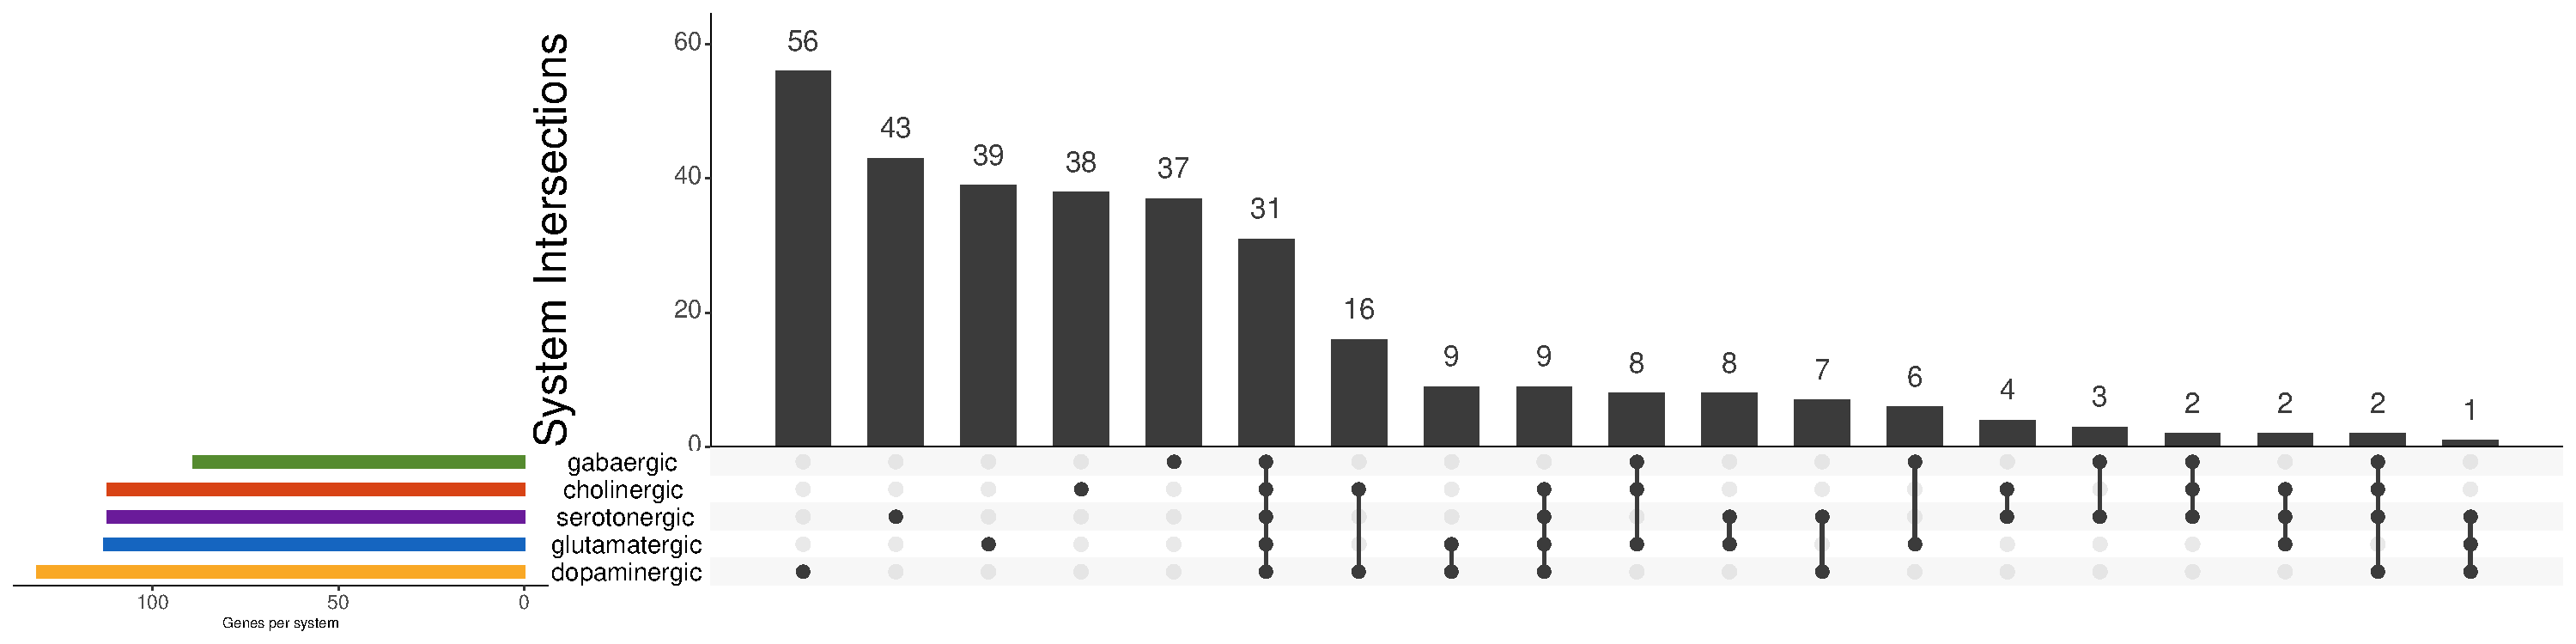
\includegraphics{figs/analysis.network.unnamed-chunk-17-1} }\newline\subfloat[Set diagram for Figure 3A\label{fig:unnamed-chunk-172}]{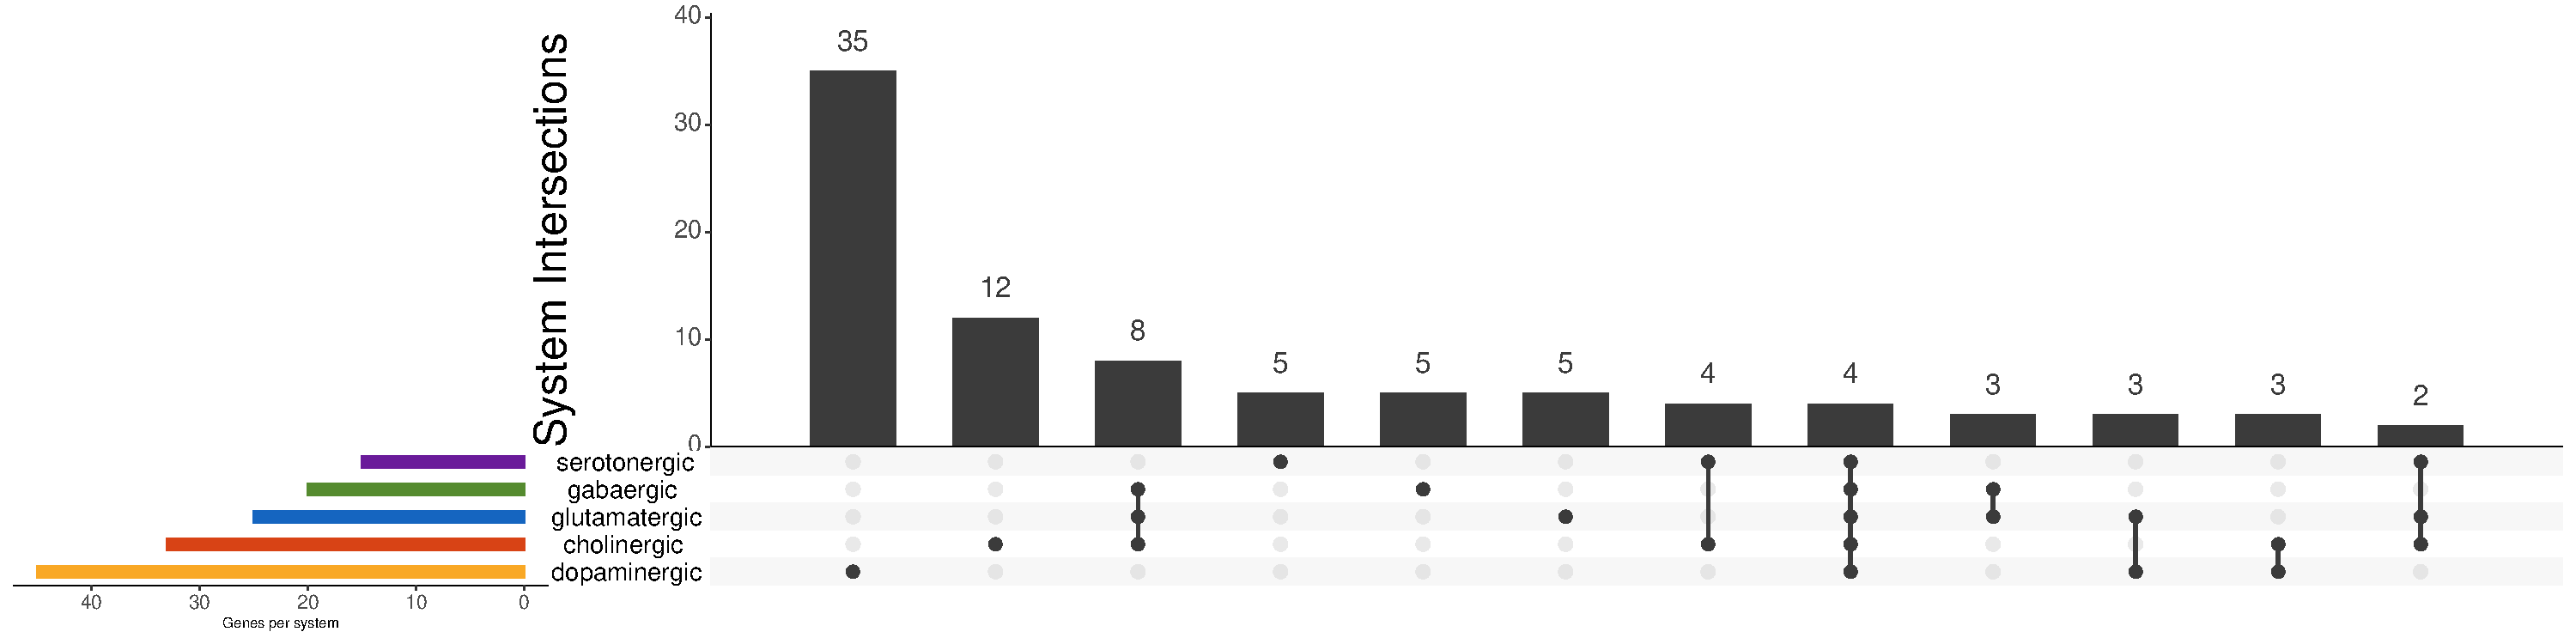
\includegraphics{figs/analysis.network.unnamed-chunk-17-2} }\newline\subfloat[Set diagram for Figure 3B\label{fig:unnamed-chunk-173}]{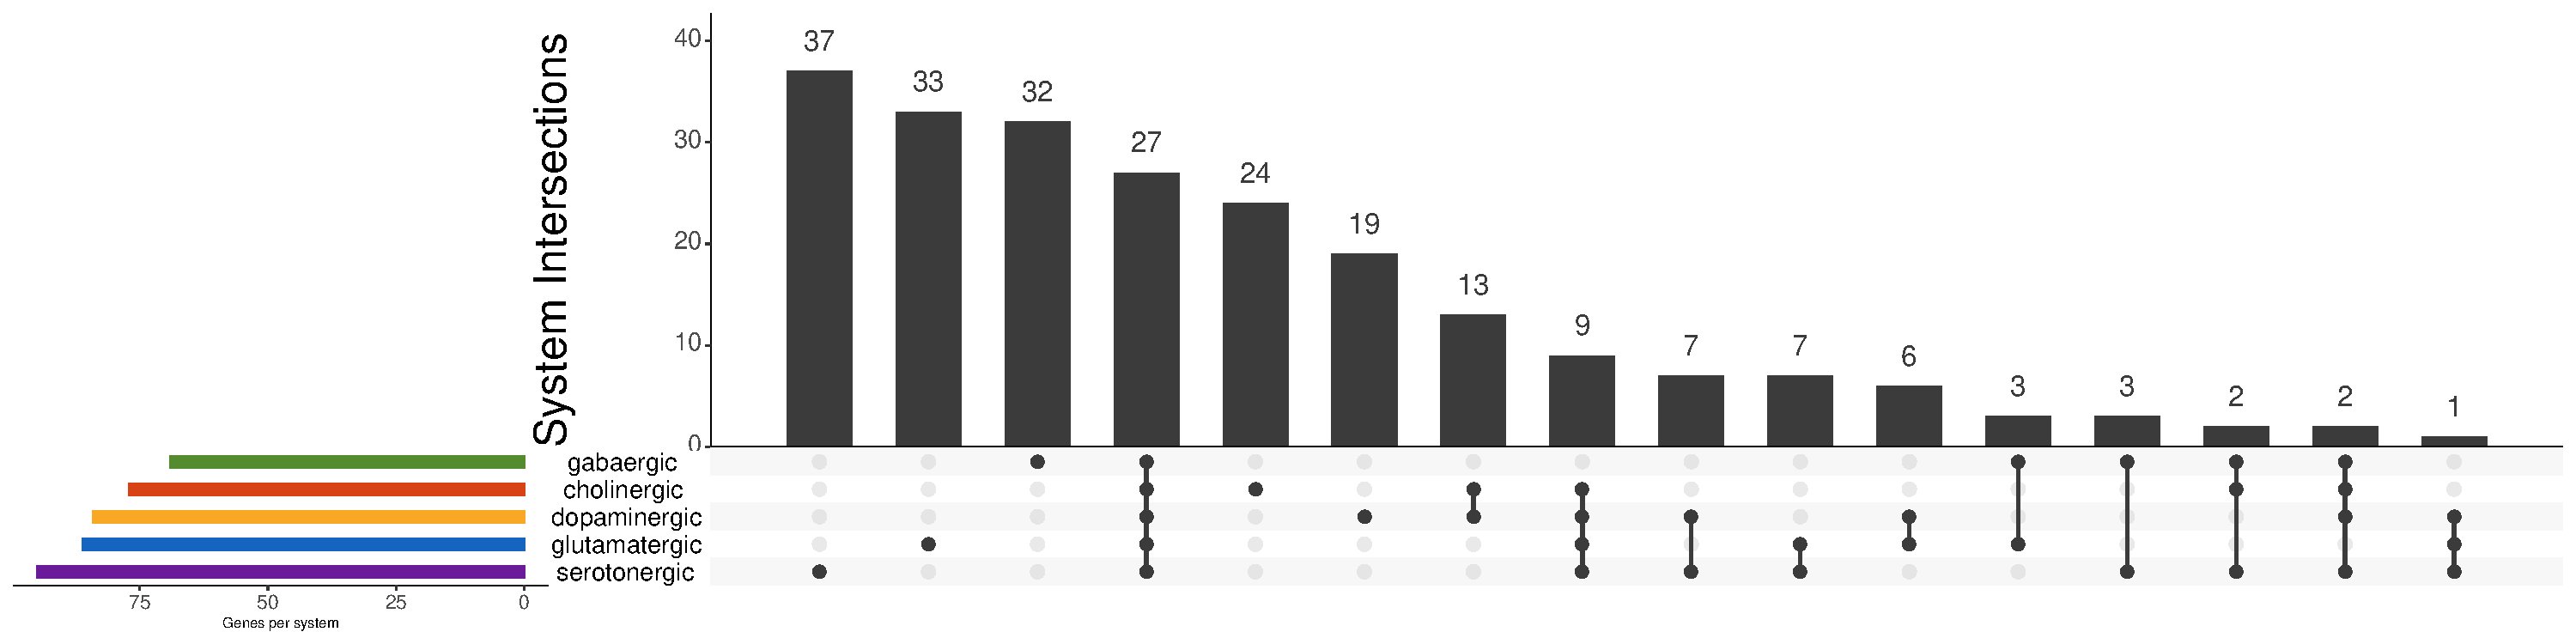
\includegraphics{figs/analysis.network.unnamed-chunk-17-3} }\caption{Set diagrams}\label{fig:unnamed-chunk-17}
\end{figure}
